% Consolidated mathematical manuscript, 18 September 2026.
% Compile twice with pdflatex from this directory after generating the figure.
\documentclass[11pt,a4paper]{article}
\usepackage[T1]{fontenc}
\usepackage[utf8]{inputenc}
\usepackage{lmodern,microtype}
\usepackage[a4paper,margin=27mm,headheight=14pt]{geometry}
\usepackage{amsmath,amssymb,amsthm,mathtools,mathrsfs}
\usepackage{graphicx,booktabs,tabularx,array,enumitem,fancyhdr,lastpage}
\usepackage[dvipsnames]{xcolor}
\definecolor{AtlasBlue}{HTML}{123E78}
\definecolor{AtlasGray}{HTML}{52616D}
\definecolor{AgendaBrown}{HTML}{694128}
\usepackage[colorlinks=true,linkcolor=AtlasBlue,citecolor=AtlasBlue,urlcolor=AtlasBlue,pdftitle={Four-Dimensional Connectedness Loci and Structural Stability for Planar Binary Similarities},pdfauthor={Bernat Espigule}]{hyperref}
\usepackage[nameinlink,noabbrev]{cleveref}
\setlength{\parskip}{3pt}
\setlength{\parindent}{14pt}
\setlength{\emergencystretch}{2em}
\renewcommand{\topfraction}{.9}
\renewcommand{\textfraction}{.05}
\renewcommand{\floatpagefraction}{.55}
\setlist{itemsep=3pt,topsep=4pt}
\renewcommand{\arraystretch}{1.13}
\newcolumntype{Y}{>{\raggedright\arraybackslash}X}
\theoremstyle{plain}
\newtheorem{theorem}{Theorem}[section]
\newtheorem{proposition}[theorem]{Proposition}
\newtheorem{lemma}[theorem]{Lemma}
\newtheorem{corollary}[theorem]{Corollary}
\theoremstyle{definition}
\newtheorem{definition}[theorem]{Definition}
\newtheorem{problem}[theorem]{Problem}
\newtheorem{example}[theorem]{Example}
\newtheorem{conjecture}[theorem]{Conjecture}
\theoremstyle{remark}
\newtheorem{remark}[theorem]{Remark}
\providecommand{\C}{\mathbb C}
\providecommand{\R}{\mathbb R}
\providecommand{\D}{\mathbb D}
\providecommand{\cK}{\mathcal K}
\providecommand{\cM}{\mathcal M}
\providecommand{\cW}{\mathcal W}
\providecommand{\id}{\operatorname{id}}
\providecommand{\eps}{\varepsilon}
\pagestyle{fancy}
\fancyhf{}
\fancyhead[L]{\sffamily\scriptsize\color{AtlasGray}CONNECTEDNESS LOCI AND STRUCTURAL STABILITY}
\fancyhead[R]{\sffamily\scriptsize\color{AtlasGray}BERNAT ESPIGUL\'E}
\fancyfoot[C]{\small\thepage}
\renewcommand{\headrulewidth}{0pt}
\title{\vspace{-1.2em}\textbf{Four-Dimensional Connectedness Loci and Structural Stability for Planar Binary Similarities}}
\author{Bernat Espigul\'e\\[.3em]\small Universitat de Girona}
\date{18 September 2026}
\begin{document}
\maketitle
\begin{abstract}
We study the connectedness loci of planar binary similarities with independently
varying contraction ratios and phases. A canonical normalization gives three
four-real-dimensional parameter spaces, according to the orientations of the
two similarities. Within this atlas, connectedness is resolved by closed
fixed-address contact fibres with exact prefix filtrations and uniform distance
bounds. Prescribed symbolic contacts define connected subfamilies; removing
their excess identifications gives a relatively $G_\delta$ stable set with a
constant coding quotient. Exact Cantor-product and parallelogram families
provide complete phase diagrams, including a discontinuous radial boundary
function. An unequal-ratio triangle family in the opposite--opposite class realizes the universal connected-core bound sharply at every contraction weight. Twelve marked binary zipper charts give smooth two-dimensional subfamilies.
A common disk bounds their stable sets; three opposite--opposite families fill
this disk exactly and have no stable islands. Finite endpoint-return criteria
certify parameter rectangles in five further presentations. Exterior coefficients
with moduli greater than one place four selected stable slices in a common
three-dimensional projection, with the fourth coordinate retained by colour.
Explicit changes of coordinates identify the Koch family underlying the wiggle island. The mathematical constructions are paired
with a real-time navigable atlas, reproducible parameter studies and independently
verifiable finite disconnection certificates. This brings complex-tree contact
families, stable slices and computational exploration into one framework while
retaining the distinction between exact classification and finite approximation.
\end{abstract}
\noindent\textbf{2020 Mathematics Subject Classification.}
Primary 28A80; Secondary 37F20, 37B10, 37M05.
\par\noindent\textbf{Keywords.}
Self-similar set; connectedness locus; planar similarity; zipper; symbolic contact;
stable set; orientation parity; exact computation.

\section{Introduction}\label{sec:introduction}
A planar self-similar set is obtained by repeatedly replacing a set by smaller
transformed copies of itself. In the binary case the attractor is the unique
nonempty compact set satisfying
\begin{equation}\label{eq:intro-ifs}
K=f_-(K)\cup f_+(K).
\end{equation}
The connectedness question becomes a problem in four real parameters when the
two contraction ratios and two complex phases vary independently. Allowing a
reflection in either map adds discrete orientation data. The purpose of the atlas
is to treat the resulting parameter loci, and the ways symbolic contacts change
along them, as mathematical objects in their own right.
Here structural stability is relative to a prescribed parameter family:
the full symbolic address-equivalence relation is exactly the relation forced
throughout that family. This is a marked coding notion, not an assertion of
ambient openness or of structural stability for a single dynamical map.

The organizing normalization places the translation constants at $-1$ and $1$.
These constants are not generally the fixed points or endpoints of the attractor.
After choosing an ordering of the maps, the two complex coefficients give a
four-real-dimensional chart for each ordered orientation type. Relabelling
identifies the two mixed types, leaving the direct--direct, direct--opposite and
opposite--opposite cases. A further reflection quotient can be taken explicitly.
This keeps coordinate identifications separate from statements about the
connectedness locus itself.

Connectedness is a first-level contact condition, but the form of that contact
varies considerably across the atlas. It can be an isolated identification,
a more complicated intersection, or an overlap compatible with a connected
attractor of positive area. A boundary point of the connectedness locus need not
have a unique touching address. The phrase \emph{just-touch frontier} will mean
the topological frontier of the connectedness locus, without an additional
assumption about contact cardinality or local smoothness.

\subsection{Background and the complex-tree programme}
Hutchinson's contraction framework gives existence, uniqueness and approximation
of self-similar attractors~\cite{Hutchinson1981}. Hata's connectedness theory
reduces the binary question to intersection of the first-level pieces~\cite{Hata1985}.
The equal-multiplier locus has a long history beginning with
Barnsley--Harrington~\cite{BarnsleyHarrington1985} and
Bandt~\cite{Bandt2002}; Calegari--Koch--Walker developed trapping and symbolic
methods in their proof of Bandt's conjecture~\cite{CalegariKochWalker2017}.
Independent complex multipliers in the direct class were studied by
Aoki--Fujimura--Taniguchi~\cite{AokiFujimuraTaniguchi2014}.
The atlas here retains both multipliers and includes opposite similarities,
while organizing exact subfamilies by their contacts and coding relations.

The present viewpoint also develops the author's work on complex trees.
Self-contact relations in symmetric tree families were studied
in~\cite{Espigule2013}. The master's thesis~\cite{Espigule2018} and the subsequent
framework~\cite{Espigule2019a} construct connected self-similar families by
prescribing identifications between symbolic addresses and then examine the
parameters at which further identifications occur. A ternary fern family is
worked out in~\cite{Espigule2019b}. The Cornell lecture in 2022 discusses
extensions of symmetric families to complex stability regions, including a
Koch-curve example~\cite[27:11--27:58]{Espigule2022Cornell}. These examples motivate a common
description of ambient connectedness loci and algebraic or analytic contact
subfamilies within them.

An interactive implementation of the three-family atlas was made publicly
available on 24 April 2026 for the author's UniLab26 workshop at the Universitat
de Girona on 25 April~\cite{Espigule2026Unilab}. It uses the four coordinates
$(\alpha,\gamma,\rho,w)$ retained here. The present account develops this
independent programme through exact subfamilies, symbolic contact loci and
computational methods.

The author's doctoral thesis~\cite{Espigule2026Thesis} develops the collinear
side of this programme through topology, finite capture and restricted
polynomial roots. The corresponding results concern specified
one-complex-dimensional families~\cite{EspiguleJuherSaldana2024,EspiguleJuher2026,Espigule2026Holes}.
Their extension to independently varying multipliers requires keeping the two
address tails and their contraction products separate. The present atlas
organizes these broader families by orientation, symbolic contact and zipper
structure.

Zippers provide another source of connected families. The endpoint conditions
give a continuous parametrization, while injectivity is an additional
property~\cite{Aseev2003,RaoZhang2019}. Calegari's wiggle family is an especially pertinent
binary zipper: its embedded-arc locus is disconnected~\cite{Calegari2026}.
The particular maps and island theorem occur in the 2022 version; the revision
of 7 September 2026 adds an explicit discussion of the two-complex-parameter
ambient family and its zipper interpretation. The coordinate comparison below
relates these presentations. Calegari--Walker~\cite{CalegariWalker2026} develop boundary dynamics,
laminations and external-angle models for the equal-multiplier family. The
relation between contact languages in the full atlas and such boundary models
is a natural further question.

\subsection{Scope and organization}
The construction has three complementary parts. First, canonical coordinates
and uniform modulus bounds organize the ambient parameter spaces. Exact
subfamilies then exhibit dust, critical contact, positive-area overlap and a
real antenna in a single parameter diagram. Second, fixed-address fibres resolve
connectedness symbolically and describe the additional identifications within
a prescribed contact family. This gives a precise connection between the atlas,
the complex-tree construction and structural stability. Third, marked zipper
charts and finite exclusion methods turn these descriptions into explicit
families and reproducible computations.

The exact classifications are given in
Corollary~\ref{cor:restored-OO-frontier} and
Theorem~\ref{thm:restored-quarter-turn}. Theorem~\ref{thm:restored-OO-triangles}
proves sharpness of the connected-core bound at every weight in the opposite--opposite
class. Theorem~\ref{thm:symbolic-contact-resolution} resolves connectedness by
fixed-address fibres, and Proposition~\ref{prop:excess-fsigma} gives the closed
filtration of excess contacts. The marked zipper surfaces are described in
Theorem~\ref{thm:zipper-surfaces}. Proposition~\ref{prop:oo00-stable-disk}
and Theorem~\ref{thm:oo01-oo10-stable-disks} classify three entire stable
slices. Proposition~\ref{prop:zipper-return-certificate} gives seven finite
return criteria. Figures~\ref{fig:zipper-stable-atlas}--\ref{fig:zipper-do-gallery}
display certified inner covers for DD$(1,0)$, DD$(1,1)$, DO$(1,0)$ and
DO$(1,1)$ in exterior coordinates and place them in the ambient atlas.
The reflected DD$(0,1)$ presentation remains part of the symbolic
dictionary. These results provide the exact structure used by the
computational companion.

The continuous geometry of the attractor, its coding relation and a finite
display label carry different information. We keep all three available in the
companion explorer. This makes the exact examples useful both as mathematical
models and as tests of numerical interpretation. The resulting contribution is
a systematic atlas with exact phase families, contact and zipper dictionaries,
and a computational method for navigating their parameter loci.

% Rigorous core for Where Fractals Just Touch.
% Standard results and elementary reductions are not claimed as new priority.
% Requires amsmath, amssymb, amsthm; theorem environments supplied by wrapper.
\providecommand{\C}{\mathbb C}
\providecommand{\D}{\mathbb D}
\providecommand{\cK}{\mathcal K}
\providecommand{\cM}{\mathcal M}
\providecommand{\cW}{\mathcal W}
\providecommand{\dist}{\operatorname{dist}}
\providecommand{\diam}{\operatorname{diam}}
\providecommand{\Fix}{\operatorname{Fix}}
\providecommand{\Ker}{\operatorname{ker}}

\section{Canonical normalization and the atlas coordinates}
\label{sec:core-normalization}

Put $J_+(z)=z$ and $J_-(z)=\overline z$. A contracting planar
similarity is $F(z)=c+\lambda J_\kappa(z)$, where
$\kappa\in\{+,-\}$ and $0<|\lambda|<1$. Its plane orientation is
$\kappa$. This discrete datum must be distinguished from the endpoint
reversal signature of a zipper, introduced below.

\begin{proposition}[Canonical translation normalization]
\label{prop:canonical-normalization}
Let $F_1,F_2$ be contracting planar similarities with distinct fixed
points. There is a unique complex-affine coordinate change
$H(z)=Az+B$, with $A\ne0$, for which
\begin{equation}\label{eq:canonical-system}
H F_1 H^{-1}(z)=-1+aJ_{\kappa_1}(z),\qquad
H F_2 H^{-1}(z)=1+bJ_{\kappa_2}(z).
\end{equation}
The coefficients satisfy $0<|a|,|b|<1$. Consequently each labelled
orientation class has the parameter domain
$\mathcal P=(\D\setminus\{0\})^2$, of real dimension four.
Pairs with a common fixed point have a singleton attractor and are
excluded from this normalization.
\end{proposition}

\begin{proof}
The real-affine map $M=(F_1+F_2)/2$ is a strict contraction, with
Lipschitz constant at most $(r_1+r_2)/2<1$. Let $c$ be its unique
fixed point and put
\[
d=F_2(c)-c=-(F_1(c)-c).
\]
If $d=0$, both similarities fix $c$, contrary to the hypothesis.
Thus $H(z)=(z-c)/d$ is an admissible coordinate change and its
conjugated maps have the stated constant terms. A direct coefficient
$\lambda$ is unchanged; an opposite coefficient becomes
$\lambda\overline d/d$, so contraction ratios and plane orientations
are preserved.

Conversely, any such normalization has to send the fixed point of
$M$ to the fixed point $0$ of the normalized average. It must also
send $F_2(c)$ to $1$. These two conditions determine $H$ uniquely.
If the original maps have a common fixed point, that singleton is
their compact invariant set, hence their attractor by uniqueness
\cite{Hutchinson1981}. Finally, the normalized maps cannot have a
common fixed point: such a point would be fixed by their average,
hence would be $0$, whereas their images of $0$ are $-1$ and $1$.
\end{proof}

We also write $S_-=S_1$ and $S_+=S_2$ for the two normalized maps.
Relabelling identifies the mixed classes $(+,-)$ and $(-,+)$,
leaving three unordered plane-orientation types $(+,+),(+,-),(-,-)$.
This is a classification of the discrete types, not an assertion
that there is only one affine-conjugacy class within each type.
In the normalized chart, relabelling followed by $z\mapsto-z$
exchanges $(a,b)$ and the orientation labels; complex conjugation
replaces $(a,b)$ by $(\overline a,\overline b)$ and preserves the
orientation labels. The normalization removes any further continuous
freedom from complex-affine conjugacy. General real-affine
coordinate changes, which may include shears, are not part of
this equivalence relation.

Write $r_1=|a|$, $r_2=|b|$. The coordinates used by the atlas are
\begin{equation}\label{eq:atlas-core-coordinates}
w=\frac{r_1}{r_1+r_2},\qquad \rho=\frac{2}{r_1+r_2},\qquad
a=\frac{2w}{\rho}e^{i(\alpha-\gamma)},\quad
b=\frac{2(1-w)}{\rho}e^{-i(\alpha+\gamma)}.
\end{equation}
Here $0<w<1$ and the strict contraction condition is
$\rho>2\max\{w,1-w\}$. The phase variables belong to a torus:
\begin{equation}\label{eq:phase-lattice}
(\alpha,\gamma)\in\mathbb R^2/\Lambda,\qquad
\Lambda=\langle(\pi,\pi),(\pi,-\pi)\rangle_{\mathbb Z}.
\end{equation}
Indeed, if $\theta_1,\theta_2$ are arguments of $a,b$, then
$\alpha=(\theta_1-\theta_2)/2$ and
$\gamma=-(\theta_1+\theta_2)/2$. One can use
$0\le\alpha\le\pi$, with $\gamma$ modulo $2\pi$, provided the seam
$(0,\gamma)\sim(\pi,\gamma+\pi)$ is retained. Endpoints of this
rectangle are not independent parameter values.

At fixed $w$, the remaining parameter domain is three-dimensional. A display
of sampled radial transitions therefore provides a way to navigate this
section of the atlas. The angular identifications in~\eqref{eq:phase-lattice}
and the sampled radial intervals are retained with each point. Section~\ref{sec:explorer-methods}
specifies the display map and its relation to the underlying parameters.



\section{Connectedness, contact and rigorous radial bounds}
\label{sec:core-connectedness}

Fix a plane-orientation type and write $S_1(z)=-1+aJ_{\kappa_1}(z)$,
$S_2(z)=1+bJ_{\kappa_2}(z)$. Let $K_p$, $p=(a,b)$, be the compact
attractor. Define
\[
\cM=\{p\in\mathcal P:K_p\text{ is connected}\},\qquad
\delta(p)=\dist(S_1K_p,S_2K_p).
\]
All parameter-space boundaries and closures below are relative to
the strict contraction domain unless another ambient space is stated.

\begin{proposition}[Binary contact criterion]\label{prop:binary-contact}
The attractor $K_p$ is connected if and only if
$S_1K_p\cap S_2K_p\ne\varnothing$, equivalently $\delta(p)=0$.
The function $\delta$ is continuous. Hence $\cM$ is relatively closed
and its complement is open.
\end{proposition}

\begin{proof}
Necessity follows because a union of two disjoint nonempty compact
sets is disconnected. For sufficiency, put $B=\operatorname{conv}(K_p)$
and $B_{n+1}=S_1B_n\cup S_2B_n$, starting at $B_0=B$.
The sets $B_n$ are nested compact sets containing $K_p$. They are
connected by induction: both images of a connected $B_n$ are
connected, and their intersection contains $S_1K_p\cap S_2K_p$.
They converge in Hausdorff distance to $K_p$, so their intersection
is connected. This is the binary instance of Hata's graph criterion
\cite{Hata1985}.

Locally in parameter space, all contraction ratios have a common
upper bound $r<1$. The associated operators on compact sets are
uniform contractions in Hausdorff distance, and their maps vary
continuously with $p$. The fixed compact sets therefore vary
continuously. Taking continuous images and then the distance between
two nonempty compact sets preserves continuity, proving the assertion
about $\delta$.
\end{proof}

\begin{proposition}[Inner and outer bounds]\label{prop:radial-bounds}
For each of the three plane-orientation types,
\begin{equation}\label{eq:modulus-bounds}
\{p:r_1^2+r_2^2\ge1\}\ \subseteq\ \cM\ \subseteq\
\{p:r_1+r_2\ge1\}.
\end{equation}
For real coefficients, in every plane-orientation type,
\begin{equation}\label{eq:real-slice}
\cM\cap(-1,1)^2=\{(a,b)\in(-1,1)^2:|a|+|b|\ge1\},
\end{equation}
with the understood exclusion of zero coefficients from $\mathcal P$.
\end{proposition}

\begin{proof}
The diameter $D_K$ of $K_p$ is positive, by distinct fixed points.
If the first two pieces intersect, their union has diameter at most
the sum of their diameters. Thus
$D_K\le(r_1+r_2)D_K$, proving the right-hand inclusion.

For the other inclusion suppose the two pieces are disjoint, with
distance $d>0$. Let $V(t)$ be the area of the open $t$-neighbourhood
of $K_p$. For $0<t<d/2$ the two corresponding neighbourhoods of the
pieces are disjoint, and similarity scaling gives
\[
V(t)=r_1^2V(t/r_1)+r_2^2V(t/r_2).
\]
For a nonempty compact planar set, $V(s)>V(t)$ whenever $s>t>0$.
For example, take a point maximizing a linear coordinate on the
compact set; a small open region beyond its $t$-supporting line lies
in the $s$-neighbourhood but outside the $t$-neighbourhood. Since
$r_j<1$, the displayed equality is incompatible with
$r_1^2+r_2^2\ge1$. This proves the left-hand inclusion, including
its equality case. It is the elementary area form of the usual
similarity-dimension obstruction to strong separation.

For real $a,b$, the real line is invariant and $K_p\subset\mathbb R$.
Let $I$ be its convex hull. The intervals $S_1I,S_2I$ have lengths
$r_1|I|,r_2|I|$, lie in $I$, and together have convex hull $I$.
Neither interval can contain both endpoints of $I$, since $r_j<1$.
Thus they cover $I$ exactly when $r_1+r_2\ge1$. In that case $I$
is a compact invariant set and equals $K_p$. Otherwise their gap
separates $S_1K_p$ from $S_2K_p$.
\end{proof}

In the atlas coordinates, these bounds read
\begin{equation}\label{eq:rho-bounds}
\rho\le2\sqrt{w^2+(1-w)^2}\ \Longrightarrow\ p\in\cM,
\qquad
p\in\cM\ \Longrightarrow\ \rho\le2.
\end{equation}
Both statements assume the strict contraction condition. Thus the
possible transition region lies between these two radii; when
$w=1/2$, they are $\sqrt2$ and $2$. This localization does not assert
that membership is monotone along every radial line.

The exact difference formulation is
\begin{equation}\label{eq:honest-difference}
D_p=aJ_{\kappa_1}(K_p)-bJ_{\kappa_2}(K_p),\qquad
p\in\cM\ \Longleftrightarrow\ 2\in D_p.
\end{equation}
It follows by rearranging the equality of a point in each first-level
piece. The product $K_p\times K_p$ is the attractor of the four
product maps $S_i\times S_j$ on $\mathbb R^4$, and $D_p$ is its
image under a real-linear projection. For unequal contraction factors
the product maps are generally self-affine. The projection does not
automatically provide a finite planar IFS for $D_p$: its evolving
relative coefficients must also be tracked. Plane-orientation parity
alone does not close that state space. Any finite graph-directed
reduction requires a separate invariance argument.


% Independently reviewed restoration from the July 2026 Encyclopedia.
% Requires the canonical normalized maps, binary contact criterion and modulus
% bounds already established in the main manuscript. No new global shell
% regularity or monotonicity is assumed.
\section{Convex support certificates and rigidity at the outer bound}
\label{sec:restored-support}

Write the normalized similarities as
\[
 f_s(z)=s+L_s z,\qquad s\in\{-1,1\},\qquad L_s=r_sO_s,
\]
where $O_s$ is an orthogonal real-linear map and $0<r_s<1$.
Put $q=\max(r_-,r_+)$, let $K$ be the attractor, and let
$P=\operatorname{conv}K$. Inner products below are the Euclidean inner
product on $\mathbb C\simeq\mathbb R^2$, with $1$ denoting the real unit
vector.

\begin{theorem}[Convex support certificate]
\label{thm:restored-support}
The support function $h(u)=\sup_{x\in P}\langle u,x\rangle$, $u\in S^1$,
is the unique continuous solution of
\begin{equation}\label{eq:restored-support-fixed}
 h(u)=\max_{s\in\{-1,1\}}
 \bigl(s\langle u,1\rangle+r_s h(O_s^{\mathsf T}u)\bigr).
\end{equation}
Define
\begin{equation}\label{eq:restored-support-gap}
 g(u)=r_-h(O_-^{\mathsf T}u)+r_+h(-O_+^{\mathsf T}u)
       -2\langle u,1\rangle.
\end{equation}
Then $f_-(P)\cap f_+(P)\ne\varnothing$ if and only if
$g(u)\ge0$ for every $u\in S^1$. In particular, one direction for which
$g(u)<0$ certifies that $K$ is disconnected.

Let $T$ denote the operator in \eqref{eq:restored-support-fixed}, and set
$h_0=0$, $h_n=T^nh_0$. Then
\begin{equation}\label{eq:restored-support-error}
 0\le h_n\le h_{n+1}\le h,\qquad
 \|h-h_n\|_\infty\le E_n:=\frac{q^n}{1-q}.
\end{equation}
If $g_n$ is obtained by replacing $h$ with $h_n$ in
\eqref{eq:restored-support-gap}, then
\begin{equation}\label{eq:restored-support-gap-error}
 g_n(u)\le g(u)\le g_n(u)+(r_-+r_+)E_n.
\end{equation}
Consequently, $g_n(u)+(r_-+r_+)E_n<0$ is a finite disconnection
certificate.
\end{theorem}

\begin{proof}
Taking the convex hull of the invariance equation gives
$P=\operatorname{conv}(f_-(P)\cup f_+(P))$. The support function of an
affine image is obtained by applying the transpose of its linear part
to the direction and adding the translation term. This proves
\eqref{eq:restored-support-fixed}. The operator $T$ is a contraction on
$C(S^1)$ in the supremum norm, with contraction constant at most $q$,
so its fixed point is unique.

The two convex pieces meet precisely when
$2\in L_-P-L_+P$. Membership in a compact convex set is equivalent to
all its supporting half-space inequalities. The support function of
$L_-P-L_+P$ is
$r_-h(O_-^{\mathsf T}u)+r_+h(-O_+^{\mathsf T}u)$, proving the criterion.
Actual first-piece contact implies convex first-piece contact.

The operator $T$ preserves pointwise order, and
$h_1(u)=|\langle u,1\rangle|\ge0$. Thus its iterates increase to $h$.
Since $\|h_1-h_0\|_\infty\le1$, the contraction estimate gives
\[
 \|h-h_n\|_\infty\le
 \sum_{j=n}^{\infty}\|h_{j+1}-h_j\|_\infty
 \le\sum_{j=n}^{\infty}q^j=E_n.
\]
Multiplying the pointwise errors by $r_-$ and $r_+$ proves
\eqref{eq:restored-support-gap-error}.
\end{proof}

\begin{remark}[Controlling unsampled directions]
\label{rem:restored-direction-grid}
Finite directional sampling also requires a bound between samples.
The function $h_n$ is the support function of the convex hull of
$\{f_u(0):|u|=n\}$, which lies in the disk of radius
$R_n=(1-q^n)/(1-q)$. Therefore $g_n$ is Lipschitz in chordal distance
on $S^1$, with constant at most
$L_n=(r_-+r_+)R_n+2$.
If every direction is within chordal distance $\eta$ of a sampled
direction, then $\min_j g_n(u_j)\ge L_n\eta$ proves convex contact.
The inequalities must use rigorous numerical enclosures when
implemented. Convex contact alone does not certify contact of the
fractal pieces; it is an outer approximation to connectedness.
\end{remark}

\begin{theorem}[Rigidity on the outer ceiling]
\label{thm:restored-outer-rigidity}
Suppose $r_-+r_+=1$. Then $K$ is connected if and only if both normalized
semilinear multipliers are real. In this case $K$ is a real interval and
$f_-(K)\cap f_+(K)$ is a singleton. Equivalently, the part of the
connectedness locus on $\rho=2$ consists precisely of these real systems.
\end{theorem}

\begin{proof}
Assume first that $K$ is connected, and put $D=\operatorname{diam}K>0$.
The level-$n$ cylinder cover has maximum diameter at most $q^nD$ and
total diameter
\[
 \sum_{|u|=n}\operatorname{diam}f_u(K)
   =D(r_-+r_+)^n=D.
\]
Hence $\mathcal H^1(K)\le D$.

We give the equality argument explicitly. Choose a diametral pair
$x,y\in K$. If $z\in K$ is not on the segment $[x,y]$, the three
strictly positive numbers
\[
 \begin{aligned}
 R_x&=\frac{|x-y|+|x-z|-|y-z|}{2},\\
 R_y&=\frac{|x-y|+|y-z|-|x-z|}{2},\\
 R_z&=\frac{|x-z|+|y-z|-|x-y|}{2}
 \end{aligned}
\]
are radii of pairwise disjoint open balls centered at $x,y,z$.
Connectedness implies that the distance from each center takes every
value between zero and the corresponding radius on the part of $K$
inside that ball. Since a distance function is $1$-Lipschitz,
\[
 \mathcal H^1(K)\ge R_x+R_y+R_z
   =\frac{|x-y|+|x-z|+|y-z|}{2}>D,
\]
a contradiction. Thus $K\subset[x,y]$, and connectedness gives
$K=[x,y]$.

It remains to identify the line. The average map
$G=(f_-+f_+)/2$ is a strict real-linear contraction fixing zero.
Convexity of the segment gives $G(K)\subset K$. Therefore
$0\in K$, and then $-1=f_-(0)$ and $1=f_+(0)$ belong to $K$.
Its supporting line is the real line. Each nonzero semilinear map
sends a nondegenerate real interval to a real interval, so its complex
multiplier is real.

Conversely, for real multipliers the real-slice criterion gives a
connected interval when $r_-+r_+=1$. The two subintervals cover $K$,
their lengths sum to the length of $K$, and they are proper
subintervals. Their intersection is consequently one point.
\end{proof}

\begin{proposition}[Area of the first-piece contact]
\label{prop:restored-contact-area}
Let $Q=f_-(K)\cap f_+(K)$ and let $m_2$ denote planar Lebesgue measure.
For every parameter,
\begin{equation}\label{eq:restored-contact-area}
 m_2(Q)=(r_-^2+r_+^2-1)m_2(K).
\end{equation}
Every point on the boundary of the connectedness locus, relative to
the strict contraction domain, satisfies
\[
 r_-+r_+\ge1,\qquad r_-^2+r_+^2\le1,
 \qquad m_2(Q)=0.
\]
If $r_-^2+r_+^2<1$, one also has $m_2(K)=0$.
\end{proposition}

\begin{proof}
Inclusion--exclusion and similarity scaling give
\[
 m_2(K)=r_-^2m_2(K)+r_+^2m_2(K)-m_2(Q),
\]
which proves the identity. The connectedness locus is relatively
closed, so a boundary point belongs to it and satisfies the outer
bound. The open set $r_-^2+r_+^2>1$ lies inside the connectedness locus
by the universal inner bound. Hence boundary points satisfy the
opposite weak inequality. If its left side is strictly less than
one, nonnegativity in \eqref{eq:restored-contact-area} forces both
measures to vanish; at equality the contact measure vanishes directly.
\end{proof}

Zero-area contact can be a nondegenerate segment. The exact families
below exhibit this on the full parameter-space boundary.

% Independently reviewed exact families restored from July 2026 material.
% All parameters satisfy strict contraction; a=0 and r=0 are excluded.
\section{Exact families across the three orientation types}
\label{sec:restored-exact-families}

For $0<t<1$, define the signed digit set
\begin{equation}\label{eq:restored-Ct}
 C_t=\left\{\sum_{n=0}^{\infty}e_nt^n:
               e_n\in\{-1,1\}\right\}.
\end{equation}
It is a Cantor set when $t<1/2$ and equals
\[
 I_t=\left[-\frac1{1-t},\frac1{1-t}\right]
\]
when $t\ge1/2$. Indeed, the intervals $-1+tI_t$ and $1+tI_t$
are disjoint for $t<1/2$ and cover $I_t$ for $t\ge1/2$.
In the first case the two maps satisfy strong separation, and
$\dim_H C_t=\log2/(-\log t)$.

\subsection{Two complete opposite--opposite families}

For $0<|a|<1$ compare the two systems
\begin{align}
 f_e(z)&=e+a\overline z,
             &&e\in\{-1,1\},\label{eq:restored-OO-diagonal}\\
 \widetilde f_e(z)&=e+ea\overline z,
             &&e\in\{-1,1\}.\label{eq:restored-OO-antidiagonal}
\end{align}
Their normalized coefficient pairs are respectively $(a,a)$ and
$(-a,a)$.

\begin{theorem}[Exact opposite--opposite phase diagram]
\label{thm:restored-OO}
Both systems have the same attractor and the same labelled geometric
first-level pieces. With $t=|a|^2$,
\begin{equation}\label{eq:restored-OO-set}
 K_a=C_t+aC_t,\qquad
 K_{a,-}=-1+tC_t+aC_t,\quad
 K_{a,+}=1+tC_t+aC_t.
\end{equation}
Their coding maps are related by a first-symbol-preserving
homeomorphism of the binary address space.

If $a\notin\mathbb R$, the following alternatives are exact.
\begin{enumerate}
\item For $|a|<2^{-1/2}$, the attractor is a real-linear image of
      $C_t\times C_t$, its two pieces are disjoint, and
      $\dim_H K_a=\log2/(-\log|a|)$.
\item For $|a|=2^{-1/2}$, the attractor is the parallelogram
      $I_t+aI_t$ and its contact set is the segment $aI_t$.
\item For $|a|>2^{-1/2}$, the attractor is the parallelogram
      $I_t+aI_t$ and its contact is the positive-area parallelogram
      \begin{equation}\label{eq:restored-OO-Q}
      Q_a=J_t+aI_t,\qquad
      J_t=\left[-\frac{2t-1}{1-t},\frac{2t-1}{1-t}\right].
      \end{equation}
\end{enumerate}
For $t\ge1/2$ their areas are
\begin{equation}\label{eq:restored-OO-areas}
 m_2(K_a)=\frac{4|\operatorname{Im}a|}{(1-t)^2},\qquad
 m_2(Q_a)=\frac{4(2t-1)|\operatorname{Im}a|}{(1-t)^2}.
\end{equation}
For real $a$, put $r=|a|$. Then $K_a=C_r$ and
\[
 Q_a=\varnothing\quad(0<r<1/2),\qquad
 Q_a=\left[-\frac{2r-1}{1-r},\frac{2r-1}{1-r}\right]
           \quad(1/2\le r<1).
\]
Thus the real transition is from a Cantor set to an interval with
point contact at $r=1/2$, and then to an interval with interval contact.
\end{theorem}

\begin{proof}
The real-linear map $A(z)=a\overline z$ satisfies $A^2=t\,\mathrm{id}$.
For the diagonal system, the coding series therefore splits as
\begin{equation}\label{eq:restored-OO-coding}
 \pi_{\mathrm{diag}}(e)
 =\sum_{k\ge0}e_{2k}t^k+a\sum_{k\ge0}e_{2k+1}t^k.
\end{equation}
The even and odd signs vary independently, proving the formula for
$K_a$. Applying either generator and using $C_t=-C_t$ gives the two
piece formulas in \eqref{eq:restored-OO-set}.

For the anti-diagonal system, its length-$n$ linear part is the
product of the first $n$ signs times $A^n$. Consequently
\[
 \pi_{\mathrm{anti}}(e)=\pi_{\mathrm{diag}}(\Phi(e)),\qquad
 \Phi(e)_n=\prod_{j=0}^n e_j.
\]
This map preserves the first symbol and is a homeomorphism: its
inverse is $e_0=d_0$ and $e_n=d_{n-1}d_n$ for $n\ge1$.
It identifies the labelled first pieces as well as the full
attractors. No commutation with the shift is asserted.

When $a$ is nonreal, $(x,y)\mapsto x+ay$ is an invertible real-linear
map. The product representation gives all asserted set types.
For $t<1/2$ the two intervals containing $-1+tC_t$ and $1+tC_t$
are separated, and linear independence of $1,a$ makes the two
planar pieces disjoint. The product has four strongly separated
similarities of ratio $t$, so its Hausdorff dimension is
$\log4/(-\log t)=\log2/(-\log|a|)$.
For $t\ge1/2$, intersecting the coordinate rectangles gives
$J_t\times I_t$. The absolute determinant of the real-linear map
is $|\operatorname{Im}a|$, giving \eqref{eq:restored-OO-areas}.

When $a$ is real, the even and odd series interleave into $C_r$;
the signs of $a$ can be absorbed into independent digit signs.
The common first pieces are $-1+rC_r$ and $1+rC_r$.
Their interval intersection gives the stated formula for $Q_a$.
\end{proof}

\begin{corollary}[Exact discontinuous radial frontier]
\label{cor:restored-OO-frontier}
Let $\mathcal M_{OO}$ be the connectedness locus in the full
four-real-dimensional opposite--opposite parameter domain. For
either embedding $\iota(a)=(a,a)$ or $\iota(a)=(-a,a)$,
\begin{align}
 \iota^{-1}(\mathcal M_{OO})
   &=\{a:2^{-1/2}\le|a|<1\}
     \cup\{a\in\mathbb R:1/2\le|a|<1\},
       \label{eq:restored-OO-connectedness}\\
 \iota^{-1}(\partial\mathcal M_{OO})
   &=\{a:|a|=2^{-1/2}\}
     \cup\{a\in\mathbb R:1/2\le|a|\le2^{-1/2}\}.
       \label{eq:restored-OO-fullboundary}
\end{align}
Writing $a=\rho^{-1}e^{i\theta}$, the connected values on a fixed ray
are exactly $1<\rho\le R(\theta)$, where
\begin{equation}\label{eq:restored-OO-radial}
 R(\theta)=
 \begin{cases}
 2,&\theta\equiv0\pmod\pi,\\
 \sqrt2,&\theta\not\equiv0\pmod\pi.
 \end{cases}
\end{equation}
\end{corollary}

\begin{proof}
The connectedness formula is the theorem. Every nonreal point of
$|a|=2^{-1/2}$ is approached along the same ray by disconnected
systems with smaller modulus. The real points on the stated
segments are approached by nonreal parameters of modulus less than
$2^{-1/2}$, also disconnected. The same construction works at the
two real endpoints of the circle. All these connected systems are
therefore boundary points of the full parameter locus.
Conversely, when $|a|>2^{-1/2}$ the strict inequality
$|a|^2+|a|^2>1$ places the parameter in the full connectedness
interior. All remaining slice parameters are disconnected, and
the disconnectedness set is open. This proves the full-boundary
formula, not just a statement about boundary relative to the slice.
Substitution of $\rho=1/|a|$ gives \eqref{eq:restored-OO-radial}.
\end{proof}

The jump is caused by the rank loss of $(x,y)\mapsto x+ay$ on the
real axis. It gives an exact example in which a radial frontier
function is discontinuous. A continuous interpolated shell can
therefore omit connected boundary segments, even on a slice whose
radial membership is completely understood.

\begin{figure}[tbp]
\centering
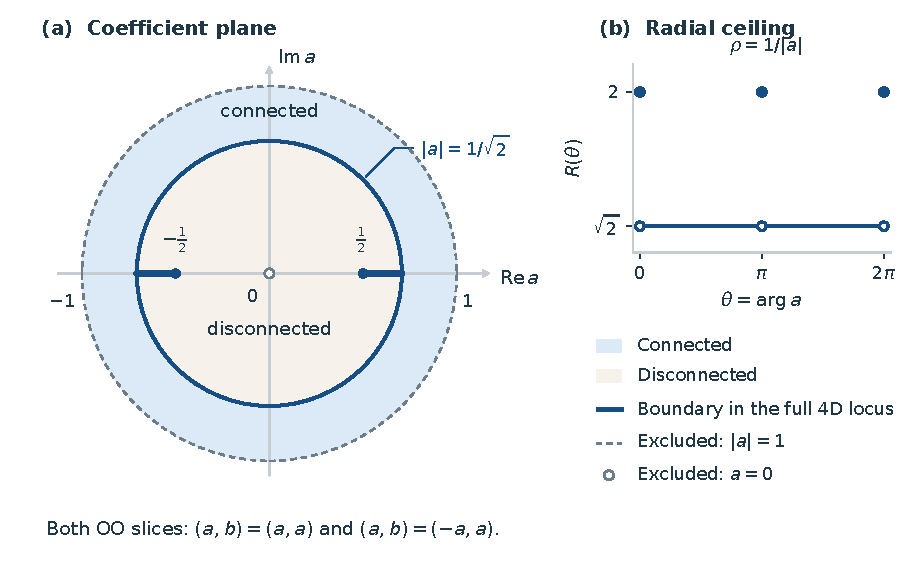
\includegraphics[width=.94\linewidth]{figures/oo_phase_diagram.pdf}
\caption{Exact opposite--opposite coefficient slices. The connected region and
its intersection with the full four-dimensional boundary follow from
Corollary~\ref{cor:restored-OO-frontier}. The real antennae produce the jumps in
the radial ceiling. The unit circle is outside the strict contraction domain.}
\label{fig:oo-phase}
\end{figure}

\subsection{A common quarter-turn family in all orientation types}

For $0<r<1$ consider the following four marked systems:
\begin{align*}
 \mathrm{DD}:&\quad f_e(z)=e+irz,\\
 \mathrm{DO}:&\quad f_-(z)=-1+irz,\qquad
                    f_+(z)=1+ir\overline z,\\
 \mathrm{OO}:&\quad f_e(z)=e+ir\overline z,\\
 \widetilde{\mathrm{OO}}:&\quad
                    f_e(z)=e+eir\overline z.
\end{align*}

\begin{theorem}[Quarter-turn equivalence across orientation types]
\label{thm:restored-quarter-turn}
All four systems have the same attractor $K_r$, the same labelled
first-level pieces, and the same geometric contact set. With
$t=r^2$,
\begin{equation}\label{eq:restored-quarter-set}
 K_r=C_t+irC_t,\qquad
 K_{r,\pm}=\pm1+tC_t+irC_t.
\end{equation}
Their coding maps are related by explicit first-symbol-preserving
homeomorphisms of the address space.

For $r<2^{-1/2}$, the attractor is a Cantor product with
$\dim_HK_r=\log2/(-\log r)$ and empty first-piece contact. At
$r=2^{-1/2}$,
\begin{equation}\label{eq:restored-quarter-critical}
 K_r=[-2,2]+i[-\sqrt2,\sqrt2],\qquad
 Q_r=i[-\sqrt2,\sqrt2].
\end{equation}
For $r>2^{-1/2}$, the attractor and its contact are the rectangles
\[
 K_r=I_t+irI_t,\qquad Q_r=J_t+irI_t.
\]
In particular, the critical parameter lies on the boundary of the
full connectedness locus in each of the three orientation types.
\end{theorem}

\begin{proof}
The two OO cases follow from Theorem~\ref{thm:restored-OO} with $a=ir$.
Use the diagonal OO coding map as the reference. In the DD case,
splitting even and odd powers of $ir$ gives
\[
 \pi_{DD}(e)=\sum_{k\ge0}(-1)^ke_{2k}t^k
              +ir\sum_{k\ge0}(-1)^ke_{2k+1}t^k.
\]
Thus $\pi_{DD}=\pi_{OO}\circ\Phi_{DD}$, where
\[
 \Phi_{DD}(e)_{2k}=(-1)^ke_{2k},\qquad
 \Phi_{DD}(e)_{2k+1}=(-1)^ke_{2k+1}.
\]
This coordinatewise involution preserves $e_0$.

For the mixed system put
$E_k=\prod_{j=0}^ke_{2j}$ and
$O_k=\prod_{j=0}^ke_{2j+1}$. A composition of two consecutive
linear parts is multiplication by $e_{2j}t$ when acting on a real
digit. Grouping these pairs, and then treating the leading odd
factor, yields
\[
 \pi_{DO}(e)=\sum_{k\ge0}E_kt^k+ir\sum_{k\ge0}O_kt^k.
\]
Equivalently, the coefficient before the digit at position $2k$ is
$E_{k-1}t^k$, and the coefficient before the digit at position
$2k+1$ is $irO_{k-1}t^k$, with empty products equal to one.
These formulas also follow directly by induction on prefix length.
Therefore $\pi_{DO}=\pi_{OO}\circ\Phi_{DO}$ with
\[
 \Phi_{DO}(e)_{2k}=E_k,\qquad
 \Phi_{DO}(e)_{2k+1}=O_k.
\]
Its continuous inverse is given by
$e_0=E_0$, $e_1=O_0$ and
$e_{2k}=E_{k-1}E_k$, $e_{2k+1}=O_{k-1}O_k$ for $k\ge1$.
This map also preserves the first symbol.

First-symbol preservation transfers the two geometric pieces and
their intersection, as well as the attractor itself. The phase
classification follows from Theorem~\ref{thm:restored-OO}.
For every one of the four presentations, approaching the critical
value with $r<2^{-1/2}$ supplies a sequence of disconnected systems in
the same orientation type. The critical system is connected, so
it lies on the full parameter-space boundary.
\end{proof}

\begin{proposition}[Address multiplicity on the critical interface]
\label{prop:restored-interface-addresses}
In any of the four critical presentations, write a contact point
as $z=iry$, where $r=2^{-1/2}$ and $-2\le y\le2$. If
$u=(y+2)/4$ is an interior dyadic rational, $z$ has four addresses;
otherwise it has two addresses, including at $y=\pm2$.
The number of address pairs $(\omega,\eta)$ representing $z$ with
$\omega_0=-1$ and $\eta_0=1$ is respectively four or one.
\end{proposition}

\begin{proof}
In the reference OO coding, zero real coordinate for an address
beginning with $-1$ forces every subsequent even digit to be $1$:
$-1+\sum_{k\ge1}e_{2k}2^{-k}=0$ attains the maximum possible tail.
An address beginning with $1$ similarly forces all subsequent even
digits to be $-1$. On either side the free odd digits code
$y=\sum_{k\ge0}e_{2k+1}2^{-k}$. This is the usual binary coding of
$u=(y+2)/4$, which has two expansions exactly at the interior
dyadic rationals and one elsewhere. Thus each side supplies two
addresses or one address, respectively. Adding counts gives four
or two total addresses; multiplying the two side counts gives
four or one cross-piece pairs. The first-symbol-preserving
recodings transfer these counts to the other presentations.
\end{proof}

This interface has uncountably many geometric contact points, even
though all but countably many of them have exactly one address
from each first piece. Geometric contact cardinality and address
multiplicity are distinct data in an atlas of connected families.

\begin{figure}[tbp]
\centering
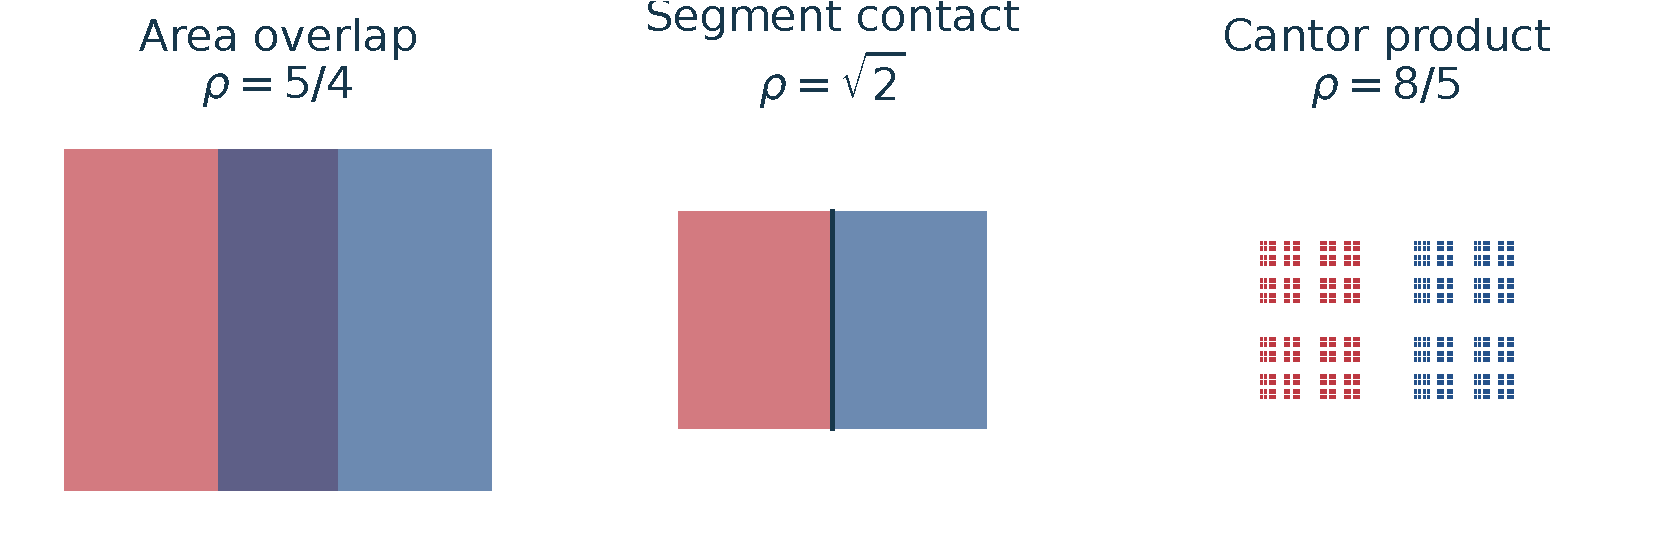
\includegraphics[width=\linewidth]{figures/quarter_turn_transition.pdf}
\caption{The common quarter-turn family of
Theorem~\ref{thm:restored-quarter-turn}, with $r=1/\rho$. Red and blue distinguish
the first-level pieces in each presentation. The first two panels are exact
rectangles and their contact. The last panel shows finite product-cylinder
covers of the Cantor attractor, using five terms in each real factor.
These are three parameter values from an exact phase classification.}
\label{fig:quarter-turn}
\end{figure}

% Restored from Encyclopedia Section 5.4; normalization and boundary proof
% independently derived. Supplies an exact family at every weight.
\subsection{Unequal-ratio triangles and sharpness at every weight}
\label{sec:restored-OO-triangles}

The preceding common quarter-turn family has equal contraction
ratios. Opposite similarities also give an exact boundary family
covering every weight $0<w<1$.

\begin{theorem}[An exact triangle on every weighted inner bound]
\label{thm:restored-OO-triangles}
Let $0<\theta<\pi/2$, put $c=\cos\theta\,e^{i\theta}$, and define
\[
 g_0(z)=c\overline z,\qquad
 g_1(z)=c+(1-c)\overline z.
\]
Their attractor is the right triangle
$T_\theta=\operatorname{conv}\{0,1,c\}$. The two pieces have disjoint
interiors and meet precisely in the altitude
$[c,\cos^2\theta]$.

The normalized opposite--opposite coefficients are
\begin{equation}\label{eq:restored-triangle-coefficients}
 a=-\cos\theta\,e^{-3i\theta},\qquad
 b=i\sin\theta\,e^{-3i\theta}.
\end{equation}
One atlas representative is
\begin{equation}\label{eq:restored-triangle-atlas}
 \alpha=\frac\pi4,\qquad
 \gamma=3\theta-\frac{3\pi}4,\qquad
 w=\frac{\cos\theta}{\cos\theta+\sin\theta},\qquad
 \rho=\frac2{\cos\theta+\sin\theta}.
\end{equation}
Every parameter in this family belongs to the boundary of the
full opposite--opposite connectedness locus and to the boundary
relative to its fixed-weight parameter space.

As $\theta$ ranges over $(0,\pi/2)$, the weight ranges over $(0,1)$,
and the boundary radius is exactly
\[
 \rho=2\sqrt{w^2+(1-w)^2}.
\]
Thus the universal connected-core bound is sharp, uniformly over
the phases, at every fixed weight in the opposite--opposite class.
\end{theorem}

\begin{proof}
Write $c=x+iy$. Then $x=\cos^2\theta$, $y=\cos\theta\sin\theta>0$,
and $x^2+y^2=x$. Direct substitution gives
\[
 g_0(0,1,c)=(0,c,x),\qquad
 g_1(0,1,c)=(c,1,x).
\]
The identity $\operatorname{Re}(c\overline{(c-1)})=0$ says that
$T_\theta$ has its right angle at $c$. The two image triangles
partition it along the altitude from $c$ to $x$. Uniqueness of
the compact invariant set gives the asserted attractor and contact.

For clarity, compute the normalization explicitly. The average map
is $G(z)=c/2+\overline z/2$, whose fixed point is
$m=x+iy/3$. With $d=g_1(m)-m$ one obtains
\[
 d=\frac y3\bigl(2y+i(1-2x)\bigr)
   =-\frac{iy}{3}e^{2i\theta},\qquad
 \frac{\overline d}{d}=-e^{-4i\theta}.
\]
Under $H(z)=(z-m)/d$, the conjugated maps have constant terms $-1$ and $1$.
An opposite multiplier $u$ becomes $u\overline d/d$; applying this
to $c$ and $1-c=-i\sin\theta\,e^{i\theta}$ proves
\eqref{eq:restored-triangle-coefficients}. The moduli and arguments
give \eqref{eq:restored-triangle-atlas}, with the usual phase-lattice
identifications.

To prove boundary membership, consider, for $0<t\le1$,
\[
 g_{0,t}(z)=tc\overline z,\qquad
 g_{1,t}(z)=c+t(1-c)\overline z.
\]
Their images of $T_\theta$ remain in $T_\theta$: they shrink the
two subtriangles toward $0$ and $c$, respectively. For $t<1$,
the first lies in $\{\operatorname{Re}z\le tx\}$ and the second
in $\{\operatorname{Re}z\ge x\}$. Since $x>0$, the two pieces
are separated. Their attractor, which lies in $T_\theta$, is
therefore disconnected.

The normalized coefficient pairs depend continuously on $t$.
Indeed, the mean-map fixed point depends continuously on $t$,
and its normalizing difference is nonzero because $g_{0,t}$ fixes
$0$ while $g_{1,t}(0)=c\ne0$. Their contraction ratios are
$t\cos\theta$ and $t\sin\theta$, so their weight is independent
of $t$, while their radius is
$2/[t(\cos\theta+\sin\theta)]$.
The disconnected normalized parameters converge to the connected
triangle as $t\uparrow1$, proving both boundary assertions.

Finally, $w=(1+\tan\theta)^{-1}$ ranges bijectively over $(0,1)$,
and
$w^2+(1-w)^2=(\cos\theta+\sin\theta)^{-2}$.
The disconnected sequence at the same weight has radii decreasing
to this inner bound. Hence no larger radius can provide a
connectedness guarantee uniformly over the phases at that weight.
\end{proof}

At $\theta=\pi/4$, the normalized coefficients are
$a=(1+i)/2$, $b=(1-i)/2$, and the normalized triangle and contact are
\[
 K=\operatorname{conv}\{-3-i,\,3-i,\,2i\},\qquad Q=[-i,2i].
\]
This supplies an exact opposite--opposite landmark at
$(\alpha,\gamma,w,\rho)=(\pi/4,0,1/2,\sqrt2)$.

\begin{figure}[tbp]
\centering
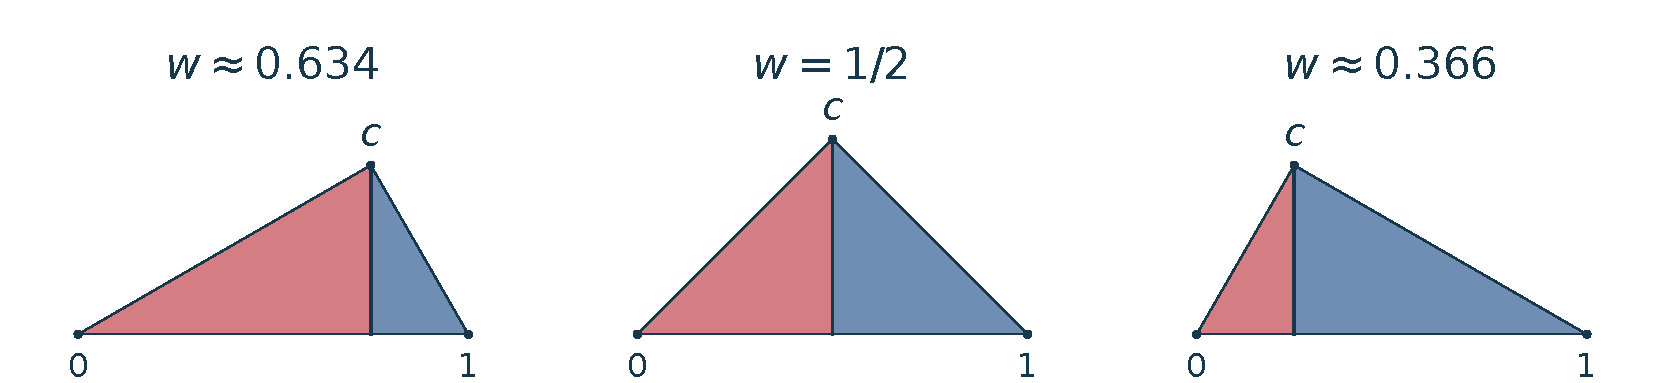
\includegraphics[width=\linewidth]{figures/triangle_contact_family.pdf}
\caption{The unequal-ratio opposite triangle family in endpoint coordinates,
with $\theta=\pi/6,\pi/4,\pi/3$. The two pieces meet along the altitude.
After canonical normalization, every triangle lies at
$\rho=2\sqrt{w^2+(1-w)^2}$; Theorem~\ref{thm:restored-OO-triangles}
proves boundary membership and sharpness for every $0<w<1$.}
\label{fig:triangles}
\end{figure}

\section{Address relations and stable families}
\label{sec:core-relations}

Let $\Sigma_m=\{1,\ldots,m\}^{\mathbb N}$, and let
$\pi_p:\Sigma_m\to K_p$ be the coding map of a contractive similarity
system. We use the following standard implication of the connectedness
criterion to specify connected families.

\begin{proposition}[Connected families from prescribed contacts]
\label{prop:prescribed-contacts}
Suppose a parameter family satisfies finitely many coding equalities
$\pi_p(i\omega)=\pi_p(j\eta)$ whose first-symbol pairs contain the
edges of a connected graph on $\{1,\ldots,m\}$. Then every attractor
in the family is connected.
\end{proposition}
\begin{proof}
The prescribed equalities give edges in the first-piece intersection
graph. To see the connectedness criterion directly, start with the
convex hull of $K_p$ and iterate the union operator, as in
Proposition~\ref{prop:binary-contact}. At each stage the images are
connected and have a connected intersection graph, since they contain
the corresponding pieces of $K_p$. The nested intersection is $K_p$.
\end{proof}

This separates enforcing connectedness from understanding additional
contacts. The complex-tree constructions in
\cite{Espigule2013,Espigule2018,Espigule2019a,Espigule2019b}
motivate treating the latter as a parameter-space problem.

\begin{proposition}[Regularity of address equations]
\label{prop:address-regularity}
For a fixed plane-orientation type, $\pi_p(\omega)$ is real analytic
in the normalized coefficients. It is holomorphic in the
direct--direct class. If $\omega$ is eventually periodic, its value
is a rational function of the coefficients and their conjugates;
in the direct--direct class it is a holomorphic rational function.
Consequently eventually periodic contact equations define relatively
real-algebraic sets, and in the direct--direct class complex algebraic
sets, after denominators are cleared. A contact equation gives a
smooth real surface in the four-dimensional chart at points where
its real Jacobian has rank two. No such rank assertion is automatic.
\end{proposition}

\begin{proof}
Write each map as $t_j+L_j$, where $t_j$ is its translation and
$L_j$ is its real-linear similarity part. The coding series is
\[
\pi_p(\omega)=t_{\omega_1}
+\sum_{n\ge1}L_{\omega_1}\cdots L_{\omega_n}t_{\omega_{n+1}}.
\]
On a compact contraction domain its terms have a geometric uniform
bound. For opposite similarities, complexify the coefficients and
their conjugates as independent variables. The same series converges
normally on a sufficiently small complex neighbourhood where all
these variables have modulus less than one. Restriction to the real
parameter domain proves real analyticity. In the direct--direct
case no conjugate variable occurs, proving holomorphic dependence.

For an address $uv^\infty$, its value is
$S_u(\Fix S_v)$. A direct affine map $c+\nu z$ has fixed point
$c/(1-\nu)$; an opposite map $c+\nu\overline z$ has fixed point
$(c+\nu\overline c)/(1-|\nu|^2)$. Word compositions have polynomial
coefficients in the original coefficients and their conjugates, and
their fixed-point denominators do not vanish under strict
contraction. This proves the rational and algebraic assertions.
The final assertion is the real implicit function theorem.
\end{proof}

For nonperiodic addresses the equations are generally analytic, not
polynomial. Nor does a contact equation by itself identify a piece
of $\partial\cM$: it can lie inside $\cM$, be a forced identity on
a connected slice, or have singular and lower-rank points.

% Optional short section: exact contact seeds, with their core location proved.
\subsection{Explicit eventually periodic contacts in the direct class}
\label{sec:restored-periodic-contacts}

Consider $f_-(z)=-1+az$ and $f_+(z)=1+bz$, with
$0<|a|,|b|<1$. Their fixed points are
$p_-=-1/(1-a)$ and $p_+=1/(1-b)$.

\begin{proposition}[Cross-contact algebraic families]
\label{prop:restored-periodic-contacts}
For every integer $k\ge1$,
\begin{equation}\label{eq:restored-periodic-criterion}
 f_-^k(p_+)=f_+^k(p_-)
 \quad\Longleftrightarrow\quad a^k+b^k=1.
\end{equation}
These parameter sets are smooth complex curves within the strict
contraction bidisk and every attractor on them is connected.
For $k\ge2$ they lie in the universal connected core
$|a|^2+|b|^2\ge1$. For $k>2$ this inequality is strict, so all such
parameters are in the interior of the full connectedness locus.
For $k=2$, equality holds only for real $a,b$.
\end{proposition}

\begin{proof}
Geometric summation and subtraction give
\[
 f_-^k(p_+)-f_+^k(p_-)
 =-\frac{(a+b-2)(a^k+b^k-1)}{(1-a)(1-b)}.
\]
The denominator is nonzero, and $a+b\ne2$ in the strict contraction
bidisk. The two points are coded by $-^k+^{\infty}$ and
$+^k-^{\infty}$, respectively, so their equality gives first-piece
contact. The gradient $(ka^{k-1},kb^{k-1})$ is nonzero, proving
smoothness of the complex curve.

If $a^k+b^k=1$, the triangle inequality gives
$|a|^k+|b|^k\ge1$. For $k\ge2$ and both moduli strictly between
zero and one,
\[
 |a|^2+|b|^2\ge |a|^k+|b|^k\ge1,
\]
with strictness in the first inequality for $k>2$.
For $k=2$, equality throughout requires $a^2$ and $b^2$ to be
nonnegative real numbers, hence $a,b$ to be real.
\end{proof}

In the atlas coordinates define
\[
 S_k(\alpha,w)=w^ke^{ik\alpha}+(1-w)^ke^{-ik\alpha}.
\]
Where $S_k\ne0$, the same contact curves have branches
\[
 \rho=2|S_k|^{1/k},\qquad
 \gamma=\frac{\arg S_k+2\pi\ell}{k},
 \quad \ell=0,\ldots,k-1,
\]
retaining only points with $\rho>2\max(w,1-w)$ and imposing the
phase-lattice identifications. These are exact connected families
with explicit contacts. For $k>2$ they cannot be frontier sheets;
their role is to provide algebraic examples and contact seeds
inside the connected region.


\subsection{Mirror symmetry and algebraic contact curves}

\begin{proposition}[Mirror-paired contacts]\label{prop:mirror-contact}
In the direct--direct chart restrict to $b=\overline a$, with
$0<|a|<1$, and let $\overline\omega$ denote the address obtained
by exchanging the two symbols of $\omega$. Then
\[
\pi_a(\overline\omega)=-\overline{\pi_a(\omega)}.
\]
The contact $\pi_a(\omega)=\pi_a(\overline\omega)$ is therefore
equivalent to the single real equation
\begin{equation}\label{eq:mirror-contact}
\Re\pi_a(\omega)=0.
\end{equation}
Every parameter satisfying this equation belongs to $\cM$.
If $\omega$ is eventually periodic, equation~\eqref{eq:mirror-contact}
is real algebraic after a nonvanishing denominator is cleared.
At a point where the gradient of its left-hand side in
$(\Re a,\Im a)$ is nonzero, its zero set is a smooth real-analytic
curve; in the eventually periodic case it is a regular branch of
a real-algebraic curve.
\end{proposition}

\begin{proof}
The reflection $R(z)=-\overline z$ satisfies $RS_1R=S_2$ and
$RS_2R=S_1$. Applying these identities to finite words and then
passing to the coding limit gives the displayed symmetry.
A point is fixed by $R$ exactly when its real part is zero, proving
\eqref{eq:mirror-contact}. The two paired addresses have opposite
first symbols, so their equality puts a point in both first-level
pieces and implies connectedness. The algebraicity assertion follows
from Proposition~\ref{prop:address-regularity}; the gradient condition
and the real-analytic implicit function theorem give the local curve.
\end{proof}

This is a precise mechanism for smooth algebraic pieces in
mirror-symmetric contact families. It does not make every such
piece a connectedness-frontier branch: contact curves may lie in
the interior of the ambient connectedness locus. For several
simultaneous address equations on the two-real-dimensional mirror
slice, one must check their effective number of independent
constraints. A single regular scalar equation, or a system of
constant rank one in a neighbourhood, gives a curve. Rank one at
one point of an arbitrary system alone does not suffice. Rank two
can give isolated solutions, while rank zero requires a separate
singularity analysis.

In the historical common-translation mirror chart
$T_1(z)=1+az$, $T_2(z)=1+\overline a z$, ordinary conjugation exchanges
the maps and the corresponding paired contact equation is
$\Im\pi_a(\omega)=0$. For nonreal $a$, canonical normalization
turns that reflection into $R(z)=-\overline z$ and preserves the
contact condition. At real $a$ the two common-translation maps
coincide, so this historical chart degenerates to a singleton;
the canonical chart should not be identified with it there.

\begin{definition}[Forced equivalences and structural stability]
For a nonempty parameter family $X$, define
\[
\mathscr R_X=\bigcap_{p\in X}\Ker\pi_p,
\qquad
\mathcal S_X=\{p\in X:\Ker\pi_p=\mathscr R_X\}.
\]
Thus $\mathscr R_X$ consists of address identifications forced
throughout the family, and $\mathcal S_X$ consists of parameters
with no additional identifications. We call this structural
stability relative to $X$; it does not assert dynamical stability
or openness in the ambient parameter space.
\end{definition}

\begin{proposition}[Topology on the stable set]
\label{prop:kernel-quotient}
For every $p\in\mathcal S_X$, the coding map induces a homeomorphism
$\Sigma_m/\mathscr R_X\to K_p$. In particular all attractors in
$\mathcal S_X$ have the same topology. Neither nonemptiness nor
openness of $\mathcal S_X$ follows from its definition.
\end{proposition}
\begin{proof}
Each coding kernel is a closed equivalence relation on compact
$\Sigma_m$, so their intersection is one also. Its quotient is
compact Hausdorff. At a parameter in $\mathcal S_X$, the induced
continuous map to $K_p$ is bijective, hence a homeomorphism.
\end{proof}


% Reconciled from Tip_point_parameter_loci_Mw_review_draft, 26 August 2026.
% Adapted to all three semilinear binary orientation classes on 18 September 2026.
% This file contains publication-facing text, not historical priority assertions.
% Requires the baseline theorem environments and macros \C, \cM, \dist.

\section{Fixed-address contact fibres and stability}
\label{sec:fixed-address-fibres}

The contact criterion can be resolved by fixing one symbolic address and
allowing its geometric image to move with the parameter. This retains the
address information that is lost when only the connectedness locus is plotted.
Throughout this section the orientation type is fixed, $p=(a,b)$ belongs to
the strict contraction domain $\mathcal P$, and
$\Sigma=\{-,+\}^{\mathbb N}$. We write $[u]$ for the cylinder with finite
prefix $u$, $\pi_p:\Sigma\to K_p$ for the coding map, and
$K_{p,u}=S_{p,u}(K_p)$. An address is denoted by $\omega$, to distinguish it
from the contraction weight $w$ of the atlas.

If $\omega_1=i$ and $j\ne i$, define the directed contact fibre and prefix locus
\begin{align}
 C_j(\omega)&=\{p:\pi_p(\omega)\in S_{p,j}(K_p)\},
 \label{eq:directed-contact-fibre}\\
 L_j(u)&=\{p:K_{p,u}\cap S_{p,j}(K_p)\ne\varnothing\},\qquad u_1=i.
 \label{eq:prefix-contact-locus}
\end{align}
Both allow every competing address beginning with $j$. This is different
from imposing an equality between two prescribed addresses, and from fixing
a spatial point independently of the parameter.

\begin{theorem}[Symbolic resolution of connectedness]
\label{thm:symbolic-contact-resolution}
The sets $C_j(\omega)$ and $L_j(u)$ are relatively closed in $\mathcal P$ and
\begin{equation}\label{eq:prefix-filtration-port}
 L_j(u)=L_j(u-)\cup L_j(u+),\qquad
 C_j(\omega)=\bigcap_{n\ge1}L_j(\omega|n).
\end{equation}
In the binary case,
\begin{equation}\label{eq:atlas-union-of-fibres}
 \cM=\bigcup_{\omega\in[-]} C_+(\omega).
\end{equation}
On a compact parameter window $P_0\subset\mathcal P$, put
$q=\max_{p\in P_0}\max\{|a|,|b|\}<1$ and $R=(1-q)^{-1}$. If
\[
 \ell_{j,\omega,n}(p)=\dist(K_{p,\omega|n},S_{p,j}K_p),\qquad
 d_{j,\omega}(p)=\dist(\pi_p(\omega),S_{p,j}K_p),
\]
then
\begin{equation}\label{eq:uniform-prefix-distance}
 0\le d_{j,\omega}(p)-\ell_{j,\omega,n}(p)\le2Rq^n.
\end{equation}
The functions $\ell_{j,\omega,n}$ increase uniformly to $d_{j,\omega}$.
\end{theorem}

\begin{proof}
The coding map is jointly continuous in the parameter and address: on any
compact window its length-$n$ truncation has error at most $Rq^n$.
The collision incidence
\[
 \{(p,\omega,\eta):\omega\in[i],\ \eta\in[j],\
       \pi_p(\omega)=\pi_p(\eta)\}
\]
is closed. Projection over the compact symbolic factors proves the
closedness assertions, including when the parameter domain is not compact.
The identity $K_{p,u}=K_{p,u-}\cup K_{p,u+}$ gives the first formula in
\eqref{eq:prefix-filtration-port}. The cylinders $K_{p,\omega|n}$ decrease
to $\{\pi_p(\omega)\}$; taking their intersections with the fixed compact
piece $S_{p,j}K_p$ gives the second formula. The first-level contact
criterion gives \eqref{eq:atlas-union-of-fibres}.
Finally $\pi_p(\omega)$ belongs to every one of its cylinders, whose
diameters are at most $2Rq^n$. Taking distance from the other first-level
piece gives \eqref{eq:uniform-prefix-distance} and monotonicity.
\end{proof}

The cover \eqref{eq:atlas-union-of-fibres} is generally not a partition:
distinct addresses can determine intersecting fibres. Over a compact
parameter window the fibre map is upper semicontinuous. Indeed, a sequence
$\omega_n\to\omega$, $p_n\to p$, with $p_n\in C_j(\omega_n)$ has a
subsequence of competing addresses converging to a competitor for $\omega$
at $p$. This statement concerns the entire fibre; it does not imply that a
selected numerical witness varies continuously.

\subsection{Inverse orbits and finite outer tests}

A word map has the form
$S_{p,u}(z)=c_{p,u}+d_{p,u}J_{\kappa_u}(z)$, with
$|d_{p,u}|$ the product of its contraction ratios. Set
\[
 h_{p,u}(\omega)=S_{p,u}^{-1}(\pi_p(\omega)).
\]
Then $p\in C_j(\omega)$ if and only if there is an address $\eta\in[j]$
for which $h_{p,\eta|n}(\omega)$ remains bounded. A competing address gives
$h_{p,\eta|n}(\omega)=\pi_p(\sigma^n\eta)$. Conversely, similarity scaling
gives
\[
 |\pi_p(\omega)-\pi_p(\eta)|
 =|d_{p,\eta|n}|\,
 |h_{p,\eta|n}(\omega)-\pi_p(\sigma^n\eta)|\longrightarrow0
\]
for every bounded inverse orbit. The argument applies equally to direct
and opposite similarities.

Let $q_p=\max\{|a|,|b|\}$, $R_p=(1-q_p)^{-1}$ and
$B_p=\overline D(0,R_p)$. Define
\[
 C_{j,N}(\omega)=\{p:\text{some }u\in\{-,+\}^N,\ u_1=j,
                        \ h_{p,u}(\omega)\in B_p\}.
\]
\begin{proposition}[Exact exhaustion and distance error]
\label{prop:fibre-exhaustion}
These sets are relatively closed and nested, and
\[
 C_j(\omega)=\bigcap_{N\ge1}C_{j,N}(\omega).
\]
If $S_{p,j,N}=\bigcup_{|u|=N,\,u_1=j}S_{p,u}(B_p)$ and
$d_{j,\omega,N}(p)=\dist(\pi_p(\omega),S_{p,j,N})$, then on $P_0$
\[
 0\le d_{j,\omega}(p)-d_{j,\omega,N}(p)\le2Rq^N.
\]
\end{proposition}
\begin{proof}
The disk is forward invariant. Thus a surviving word has surviving prefixes,
and the finite survivor sets decrease. If every depth has a survivor,
K\"onig's lemma gives an infinite branch with bounded inverse orbit, which
is a competing address by the preceding argument. Conversely every true
competitor survives. Finite unions of the continuous closed inequalities
$|h_{p,u}(\omega)|\le R_p$ prove closedness. The nested compact sets
$S_{p,j,N}$ contain $S_{p,j}K_p$ and approximate it in Hausdorff distance
within $2Rq^N$, proving the distance estimate.
\end{proof}

If an arbitrary address is evaluated using
$\widehat\pi_{p,L}(\omega)=S_{p,\omega|L}(0)$, its error is at most $Rq^L$.
After inversion along $u$, the error is at most $Rq^L/|d_{p,u}|$.
Consequently the strict inequality
\begin{equation}\label{eq:fibre-safe-pruning}
 \dist\bigl(S_{p,u}^{-1}(\widehat\pi_{p,L}(\omega)),B_p\bigr)
       >\frac{Rq^L}{|d_{p,u}|}
\end{equation}
is a sound pruning test when evaluated with validated numerical bounds.
Finite survival retains an outer approximation. Membership requires a
positive certificate, such as an exact equality with a competing address;
when both addresses are eventually periodic their values can be evaluated
exactly by the corresponding fixed-point formulas.

\subsection{Forced contacts and the stable set of a subfamily}

Let $X\subset\mathcal P$ be a nonempty subfamily. Put
\[
 \mathscr Q_p=\{(\omega,\eta)\in\Sigma^2:\omega_1\ne\eta_1,
                         \ \pi_p(\omega)=\pi_p(\eta)\},\qquad
 \mathscr Q_X=\bigcap_{p\in X}\mathscr Q_p.
\]
The relation $\mathscr Q_X$ consists of the first-level contacts forced throughout
the family. The excess fibre associated with an address is
\[
 M_X(\omega)=\{p\in X:\text{some }\eta\text{ satisfies }
                        (\omega,\eta)\in \mathscr Q_p\setminus \mathscr Q_X\}.
\]
This is the tip-point construction relative to the prescribed contact
structure. It coincides with the full contact fibre when $\mathscr Q_X$ is empty.
For a zipper surface, $\mathscr Q_X$ already includes its endpoint identifications,
so $M_X(\omega)$ records additional identifications rather than the contact
that makes the whole surface connected.

\begin{proposition}[Closed approximation of excess instability]
\label{prop:excess-fsigma}
The excess-instability locus
$U_X=\bigcup_{\omega\in\Sigma}M_X(\omega)$ is an $F_\sigma$ subset of $X$.
Every fixed-address excess fibre is $F_\sigma$ as well. The structural
stable set $\mathcal S_X=\{p\in X:\Ker\pi_p=\mathscr R_X\}$ is
$X\setminus U_X$ and hence is $G_\delta$ in $X$.
\end{proposition}
\begin{proof}
If $\mathscr Q_X=\varnothing$, the excess locus is the relatively closed
connectedness locus restricted to $X$, and each excess fibre is relatively
closed. Otherwise choose any compatible metric on the compact space
$\Sigma^2$. For $m\ge1$ put
\[
 U_{X,m}=\{p\in X:\exists(\omega,\eta)\in \mathscr Q_p,
                        \ d((\omega,\eta),\mathscr Q_X)\ge1/m\}.
\]
The set $\mathscr Q_X$ is closed and compact. The collision equation, the different
first symbols and the distance constraint are closed conditions;
projection over the compact symbolic space makes $U_{X,m}$ relatively
closed in $X$. These sets increase and their union is $U_X$, since each
nonpersistent pair has positive distance from $\mathscr Q_X$. Fixing $\omega$
gives the same filtration for $M_X(\omega)$.

Finally, every nontrivial equal-address pair has a finite common prefix.
Removing that prefix, using injectivity of its word map at every parameter,
gives a pair with different first symbols. The original equality is forced
throughout $X$ exactly when its reduced equality is. Thus there are no
excess first-level pairs exactly when the full coding kernel equals
$\mathscr R_X$, proving the assertion about $\mathcal S_X$.
\end{proof}

This descriptive regularity does not assert openness or nonemptiness.
It complements the quotient description of the stable attractors:
the connectedness locus is resolved by closed contact fibres, whereas the
stable set of a prescribed contact family is obtained by removing its
excess identifications.

\subsection{Two exact contact curves in the mirror family}

The historical complex-tree chart provides explicit examples with one
complex parameter. Consider
$T_1(z)=1+cz$, $T_2(z)=1+\overline c z$, $0<|c|<1$.
For the first pair of addresses,
\[
 \pi_c(12^\infty)-\pi_c(21^\infty)
   =\frac{(c-\overline c)(1-c-\overline c)}
          {(1-c)(1-\overline c)}.
\]
For the second pair,
\[
 \pi_c(122(21)^\infty)-\pi_c(211(12)^\infty)
 =\frac{(c-\overline c)
        \bigl(1-2|c|^2-|c|^2(c+\overline c)\bigr)}{1-|c|^2}.
\]
Both identities follow by summing the finite prefix and geometric period.
Away from the real axis their zero sets are respectively
\begin{equation}\label{eq:mirror-two-curves-port}
 \Re c=\tfrac12,\qquad 2|c|^2(1+\Re c)=1.
\end{equation}
The upper branch of the second curve is smooth: with $c=x+iy$ its
defining function has $y$-derivative $4y(1+x)>0$ when $y>0$ and $|c|<1$.
Each curve is contained in the corresponding fixed-address contact fibre.
Neither equality alone asserts that it exhausts that fibre or lies on
the ambient connectedness frontier. At real $c$ the two historical maps
coincide; this is the chart degeneration already distinguished from the
canonical binary normalization.

\section{Zippers: endpoint structure and the binary atlas}
\label{sec:core-zippers}

The endpoint signature and the plane-orientation type are independent.
To keep their roles explicit, use bits $e_j\in\{0,1\}$ for endpoint
reversal and signs $\kappa_j\in\{+,-\}$ for plane orientation.

\begin{proposition}[General planar similarity zippers]
\label{prop:general-zipper}
Let $z_0=0,z_1,\ldots,z_m=1$ satisfy
$0<|z_j-z_{j-1}|<1$, and prescribe $e_j,\kappa_j$. The maps
\begin{equation}\label{eq:general-zipper}
F_j(t)=z_{j-1+e_j}+(-1)^{e_j}(z_j-z_{j-1})J_{\kappa_j}(t)
\end{equation}
form a zipper. For any partition
$0=t_0<t_1<\cdots<t_m=1$, there is a unique continuous map
$\zeta:[0,1]\to\C$ with $\zeta(0)=0,\zeta(1)=1$ such that
\[
\zeta\circ h_j=F_j\circ \zeta,
\]
where $h_j$ maps $[0,1]$ affinely onto $[t_{j-1},t_j]$ and reverses
endpoint order exactly when $e_j=1$. Its image is the IFS attractor.
Conversely, every planar similarity zipper with marked ordered
endpoints and vertices takes this form after endpoint normalization.
\end{proposition}
\begin{proof}
Formula~\eqref{eq:general-zipper} maps its ordered endpoints to
$z_{j-1},z_j$ with the indicated reversal. Define an operator on
the complete space of continuous maps with endpoint values $0,1$
by $(T\zeta)\circ h_j=F_j\circ \zeta$. The endpoint identities ensure that
the pieces agree at every partition point and retain the outer
endpoints. Its sup-norm contraction ratio is
$\max_j|z_j-z_{j-1}|<1$, so it has a unique fixed map $\zeta$.
The compact set $\zeta([0,1])$ is invariant under the IFS, and therefore
is its attractor. Conversely, an endpoint-normalized similarity has
coefficient and translation determined by its two endpoint values
and its plane orientation, giving the formula.
\end{proof}

This is the standard zipper construction \cite{Aseev2003}. It
covers any finite number of maps, but only the binary case lies
in the four-dimensional atlas. An attractor that is a Jordan arc
does not necessarily make its given generators a zipper: the two
interval maps $0.6t$ and $0.6t+0.4$, for instance, have attractor
$[0,1]$ with an overlap interval between their pieces.

Let $\tau:\Sigma_m\to[0,1]$ be the coding map for $h_j$. Then
$\pi_p=\zeta_p\circ\tau$, so $\Ker\tau\subseteq\Ker\pi_p$ for every
zipper with this partition and endpoint signature. The canonical
zipper curve is embedded exactly when these kernels are equal.
This distinguishes the canonical embedded-curve locus from the
weaker property that the unparameterized attractor happens to be
a Jordan arc. It also gives a precise meaning to having only the
prescribed endpoint identifications.

For $m=2$, write $q=z_1$ and
$\Omega=\{q:|q|<1,\ |1-q|<1\}$. Formula~\eqref{eq:general-zipper}
becomes
\begin{equation}\label{eq:binary-endpoint-zipper}
F_1(t)=e_1q+(-1)^{e_1}qJ_{\kappa_1}(t),\qquad
F_2(t)=q+e_2(1-q)+(-1)^{e_2}(1-q)J_{\kappa_2}(t).
\end{equation}
Thus each fixed binary signature and plane-orientation choice has
one complex endpoint parameter, independently of the full four-real-
dimensional parameter domain of binary systems.

\begin{theorem}[The binary zipper surfaces]\label{thm:zipper-surfaces}
Fix the plane-orientation type and an endpoint signature
$e=(e_1,e_2)$. Within the canonical translation chart, the systems
admitting this marked ordered zipper structure form an embedded
real-analytic surface parametrized by $q\in\Omega$. It is relatively
real algebraic. In the direct--direct class these four surfaces are
exactly
\begin{equation}\label{eq:four-planes}
\begin{array}{c|c}
(e_1,e_2)&\text{coefficient equation}\\\hline
(0,0)&a+b=1\\
(0,1)&a-b=1\\
(1,0)&-a+b=1\\
(1,1)&a+b=-1.
\end{array}
\end{equation}
For the other plane-orientation types, the same equations hold in
the endpoint coefficient chart defined in the proof, but need not
be literal affine planes in the canonical translation coefficients.
\end{theorem}

\begin{proof}
For an arbitrary normalized pair $S_1,S_2$, the outer endpoints
$u,v$ required by the selected signature are uniquely determined:
\[
\begin{array}{c|cc}
e&u&v\\\hline
(0,0)&\Fix S_1&\Fix S_2\\
(0,1)&\Fix S_1&S_2(u)\\
(1,0)&S_1(v)&\Fix S_2\\
(1,1)&\Fix(S_1S_2)&S_2(u).
\end{array}
\]
They are distinct: equality in any row would give a common fixed
point of $S_1,S_2$. Set $d=v-u$ and conjugate by $t\mapsto u+dt$.
The two maps in these endpoint coordinates have the form
\begin{equation}\label{eq:endpoint-chart}
\widehat S_1(t)=A J_{\kappa_1}(t)-e_1A,\qquad
\widehat S_2(t)=B J_{\kappa_2}(t)+1-(1-e_2)B,
\end{equation}
where $A=a$ for $\kappa_1=+$ and
$A=a\overline d/d$ for $\kappa_1=-$, and similarly for $B$.

For each signature, the transformation $(a,b)\mapsto(A,B)$ is a
real-analytic diffeomorphism of the punctured contraction bidisk. To prove
surjectivity and the inverse, start with arbitrary $(A,B)$ in the
punctured bidisk and the maps~\eqref{eq:endpoint-chart}. The indicated outer
endpoint identities hold at $0,1$. These maps cannot have a common
fixed point: in each of the four rows the unique fixed points or
alternating two-cycle force the distinct outer endpoints. Apply
Proposition~\ref{prop:canonical-normalization} to recover a canonical
pair. Taking its signature endpoints returns the original chart,
so the two constructions are inverse. All fixed-point operations
are real rational by the formulas in
Proposition~\ref{prop:address-regularity}. The average-map fixed
point used in canonical normalization is also real rational: if
its linear part is $cz+d\overline z$, then $|c|+|d|<1$, and its
fixed point is obtained by an invertible two-by-two real linear
system. Thus these inverse changes of chart are real rational,
with no vanishing denominator in the contraction domain.

The two inner endpoints in~\eqref{eq:endpoint-chart} agree exactly
when
\[
(-1)^{e_1}A+(-1)^{e_2}B=1.
\]
This is a smooth complex affine plane intersected with the bidisk,
parametrized by $A=(-1)^{e_1}q$ and
$B=(-1)^{e_2}(1-q)$ for $q\in\Omega$. Pulling back through the
real-rational diffeomorphism proves the surface and algebraicity
assertions. In the direct--direct class $A=a,B=b$, which gives
\eqref{eq:four-planes}.
\end{proof}

\begin{proposition}[Embedded binary zippers]\label{prop:binary-embedding}
For the binary zipper~\eqref{eq:binary-endpoint-zipper}, its canonical
curve $\zeta$ is injective if and only if
$F_1K\cap F_2K=\{q\}$.
\end{proposition}
\begin{proof}
Necessity follows by applying injectivity to the two closed
partition intervals. Conversely suppose the intersection is
$\{q\}$. Since $q\ne0,1$, the point $0$ belongs only to the first
piece, and $1$ only to the second. Let $E_j=\zeta^{-1}(j)$ for $j=0,1$.
The endpoint equations express each $E_j$ as an affine contracting
image, under an appropriate interval map $h_i$, of one of $E_0,E_1$.
For signature $(0,0)$ both sets are self-images; for $(0,1)$ the
first is a self-image and determines the second; for $(1,0)$ the
reverse holds; and for $(1,1)$ composing the two equations gives
a strict contracting self-image for each set. In all cases
compactness gives $E_0=\{0\}$ and $E_1=\{1\}$, using the prescribed
endpoint values.

If two different interval parameters had the same image, remove
their longest common interval-cylinder prefix. At the first
separation their images lie in the two first-level pieces, hence
equal $q$. Inverting the corresponding injective planar map sends
this equality to an endpoint. At least one preimage parameter is
not the partition endpoint, contradicting the uniqueness just
proved. Hence $\zeta$ is injective.
\end{proof}

All binary zipper surfaces lie in $\cM$, regardless of embeddedness.
For $q\in(0,1)$, the endpoint maps act on the real interval as two
consecutive subinterval maps; their canonical curve is a
homeomorphism. Thus over a whole binary zipper surface the forced
kernel is exactly $\Ker\tau$, and its structural stable set is
the canonical embedded-zipper locus. This does not prove that this
locus is connected, or that its components remain distinct after
leaving the surface.

\subsection{The wiggle slice and the historical tree chart}

For plane orientation $(+,+)$ and endpoint signature $(1,1)$,
equation~\eqref{eq:binary-endpoint-zipper} gives Calegari's maps
\[
f_q(t)=-qt+q,\qquad g_q(t)=(q-1)t+1.
\]
Their canonical translation coefficients are $a=-q,b=q-1$.
More explicitly, with $Q(q)=q^2-q+1$,
\[
H_q(t)=\frac{3t-(1+q)}{Q(q)}
\]
conjugates this pair to $-1-qt$ and $1+(q-1)t$.
The zeros of $Q$ are $(1\pm i\sqrt3)/2$, on the excluded
contraction boundary, so this change is valid throughout $\Omega$.
Calegari proves that the embedded-curve locus on this slice is
disconnected \cite{Calegari2026}. Every attractor on the slice is
connected; the disconnected locus in that result is a parameter
space of embeddings, not a family of disconnected attractors.

The common-translation complex-tree maps $1-qt$ and $1+(q-1)t$
are conjugate to $f_q,g_q$ through
\[
J_q(t)=\frac{(q^2-q+1)t+q-1}{2q-1},\qquad q\ne\tfrac12.
\]
At $q=1/2$ the tree maps coincide and their attractor is
$\{2/3\}$; the endpoint-normalized wiggle remains $[0,1]$.
This is a genuine chart degeneration. It does not affect the
identification at nonreal island parameters, but must be retained
when comparing the entire families. Disconnectedness of an
embedded-curve locus on this two-dimensional surface does not
imply disconnectedness of an embedding locus in the ambient atlas.


\subsection{Stable slices of the twelve marked families}
\label{sec:stable-zipper-slices}

For each plane-orientation choice $\kappa$ and endpoint signature $e$, let
\[
 \mathcal S_{\kappa,e}
 =\{q\in\Omega:F_{1,q}K_q\cap F_{2,q}K_q=\{q\}\}.
\]
This is the stable set of that marked zipper surface. The parameters in
$\Omega\setminus\mathcal S_{\kappa,e}$ still give connected attractors;
their canonical curves have additional identifications. In particular,
these plots resolve structure \emph{within} the connectedness loci.
The signs of $\kappa$ describe orientation in the plane, while the bits of
$e$ describe traversal of the two curve pieces.

\begin{proposition}[A common necessary disk]
\label{prop:zipper-necessary-disk}
For every marked binary planar zipper,
\[
 (0,1)\subset\mathcal S_{\kappa,e}
 \subset \mathbb D_{1/2}:=\{q:|q-\tfrac12|<\tfrac12\}.
\]
\end{proposition}
\begin{proof}
The real interval was established above. If the canonical curve is
embedded, its two pieces meet in one point. The planar finite-intersection
theorem of Bandt and Rao~\cite{BandtRao2007} therefore gives the open set
condition. Choose a bounded nonempty feasible open set $O$ (intersect a feasible open
set with a sufficiently large forward-invariant open ball) and write
$r_1=|q|$, $r_2=|1-q|$. The disjoint sets $F_1(O),F_2(O)\subset O$ imply
$r_1^2+r_2^2\le1$ by planar area. Equality is impossible for a Jordan arc:
in that case $O\setminus\bigcup_{|u|=n}F_u(O)$ has area zero for every $n$,
so the latter union is dense in $O$. Its distance from $K$ tends uniformly
to zero as $n\to\infty$, which implies $O\subset K$. An arc has empty
interior. Hence $|q|^2+|1-q|^2<1$, equivalent to the displayed disk.
\end{proof}

In the atlas coordinates this necessary disk is
$\rho>2\sqrt{w^2+(1-w)^2}$. Stable zipper parameters therefore lie between
the guaranteed connected core and the outer bound $\rho\le2$; the real
interval occupies $\rho=2$.

\begin{proposition}[An exact reversing zipper slice]
\label{prop:oo00-stable-disk}
For $\kappa=(-,-)$ and $e=(0,0)$, the stable set is exactly
$\mathcal S_{--,00}=\mathbb D_{1/2}$. If $q\notin\mathbb R$ lies on its
boundary circle, the attractor is the filled triangle
$T_q=\operatorname{conv}\{0,q,1\}$ and the two pieces meet in the segment
$[q,|q|^2]$.
\end{proposition}
\begin{proof}
Conjugation permits $\Im q>0$. Put $x=\Re q$ and $s=|q|^2$. The maps are
$F_1(z)=q\overline z$ and $F_2(z)=q+(1-q)\overline z$, and their triangle
images are
\[
 F_1(T_q)=\operatorname{conv}\{0,q,s\},\qquad
 F_2(T_q)=\operatorname{conv}\{q,1,2x-s\}.
\]
The strict contraction lens ensures $0<s<1$ and $0<2x-s<1$, so both images
are contained in $T_q$. When $q\in\mathbb D_{1/2}$, we have $s<x$;
the base intervals $[0,s]$ and $[2x-s,1]$ are disjoint and the triangles
meet only at $q$. Thus $K_q\subset T_q$ and its first-level pieces meet
only at $q$, proving embeddedness. For real $q\in(0,1)$ the attractor is
the interval and embeddedness follows directly. The necessary-disk
proposition excludes every remaining parameter. On the nonreal circle
$s=x$, the two triangles exactly tile $T_q$ and share the segment from
$q$ to $s$; uniqueness of the attractor gives the asserted filled triangle.
\end{proof}

\subsection{Two further exact stable disks}
\label{subsec:oo01-oo10-exact-disk}

The opposite--opposite endpoint signatures $01$ and $10$ have the
same complete stable disk as signature $00$. In particular, these
families supply exact cases with no stable islands.

\begin{theorem}[Exact stable disks for the reversing signatures $01$ and $10$]
\label{thm:oo01-oo10-stable-disks}
For the opposite--opposite binary zippers with endpoint signatures
$e=(0,1)$ and $e=(1,0)$,
\[
 \mathcal S_{--,01}=\mathcal S_{--,10}
 =\left\{q:\left|q-\frac12\right|<\frac12\right\}.
\]
Put $s=|q|^2$ and $t=|1-q|^2$. In the $01$ case an invariant
triangle on the stable disk is
\[
 T_{01}(q)=\operatorname{conv}\left\{0,1,\frac{q}{1-t}\right\};
\]
in the $10$ case it is
\[
 T_{10}(q)=\operatorname{conv}\left\{0,1,\frac{q-s}{1-s}\right\}.
\]
For nonreal $q$ on the boundary circle $s+t=1$, the respective
attractors are these filled triangles. The first-level intersection
is $[q,1]$ for signature $01$, and $[0,q]$ for signature $10$.
\end{theorem}
\begin{proof}
Consider signature $01$, whose maps are
\[
 F_1(z)=q\overline z,\qquad
 F_2(z)=1-(1-q)\overline z.
\]
Complex conjugation permits $\Im q=y>0$. The real interval
$q\in(0,1)$ gives an embedded interval directly. Define
\[
 C=\frac{q}{1-t},\qquad A=\frac{s}{1-t}.
\]
The contraction lens gives $0<t<1$. A direct calculation gives
\[
 F_2^2(z)=q+tz,\qquad F_2(C)=C,
\]
and hence
\begin{align*}
 F_1(T_{01})&=\operatorname{conv}\{0,q,A\},\\
 F_2(T_{01})&=\operatorname{conv}\{1,q,C\}.
\end{align*}
Inside the disk, $s+t<1$, so $0<A<1$ and
$q=(1-t)C$ lies strictly between $0$ and $C$. Every displayed vertex
therefore lies in $T_{01}$, proving invariance.

The line through $q$ and $1$ separates these two image triangles.
More explicitly, the real-linear functional
\[
 \ell(z)=\Im\bigl(\overline{(1-q)}(z-q)\bigr)
\]
obeys
\[
 \ell(0)=-y<0,\quad
 \ell(A)=(A-1)y<0,\quad
 \ell(q)=\ell(1)=0,\quad
 \ell(C)=\frac{t}{1-t}y>0.
\]
Thus $F_1(T_{01})$ meets the separating line only at $q$, while
$F_2(T_{01})$ lies on the other closed side. Their intersection is
exactly $\{q\}$. The attractor lies in $T_{01}$, so its first-level
pieces also meet exactly at their prescribed join. The binary
embedding criterion proves embeddedness throughout the disk.
The common necessary-disk theorem excludes every remaining parameter
in the contraction lens.

On the nonreal boundary $s+t=1$, one has $A=1$. The two image
triangles then partition $T_{01}$ along $[q,1]$ because $q$ lies on
the side $[0,C]$. Consequently their union is $T_{01}$, and uniqueness
of the attractor gives the asserted filled triangle and overlap.

Finally, endpoint reflection $z\mapsto1-z$ with generator exchange
sends signature $01$ at $1-q$ to signature $10$ at $q$. It sends
$T_{01}(1-q)$ to
\[
 \operatorname{conv}\left\{0,1,
 1-\frac{1-q}{1-s}\right\}
 =T_{10}(q)
\]
and sends the shared boundary segment $[1-q,1]$ to $[0,q]$.
\end{proof}

The finite return tests below also apply to these signatures, but the
triangle proof already classifies their complete stable sets.


\paragraph{Finite certificates in seven marked slices.}
A common endpoint return turns the prescribed contact into a finite
verification. Word maps are composed from left to right in symbolic order,
so $F_{12}=F_1\circ F_2$. The following table gives seed words $U,V$,
return words $r,s$, and the multiplier $\eta$ of a common similarity
$H(z)=q+\eta(z-q)$ satisfying
\begin{equation}\label{eq:zipper-return-identities}
 F_{Ur}=H\circ F_U,\qquad F_{Vs}=H\circ F_V.
\end{equation}
Every row holds identically on the contraction lens.
\begin{center}
\begin{tabular}{cc|cc|cc|c}
Plane type&$e$&$U$&$V$&$r$&$s$&$\eta$\\\hline
DD&01&12&22&1&1&$q$\\
DD&10&11&21&2&2&$1-q$\\
DD&11&1&2&12&21&$q(1-q)$\\
DO&10&11&21&22&22&$|1-q|^2$\\
DO&11&1&2&1212&2121&$|q|^2|1-q|^2$\\
OO&01&12&22&11&11&$|q|^2$\\
OO&10&11&21&22&22&$|1-q|^2$
\end{tabular}
\end{center}
Here DO means that $F_1$ is direct and $F_2$ opposite. The identities follow
by composition; in the rows with a reversing endpoint return, taking its
square produces the displayed positive real multiplier. Since $|\eta|<1$,
$H$ is a strict contraction fixing the join.

\begin{proposition}[A finite certificate for an embedded zipper]
\label{prop:zipper-return-certificate}
Fix one row of the table, put $d=|U|=|V|$ and $m=|r|=|s|$, and suppose:
\begin{enumerate}
\item among the pairs $F_uK\cap F_vK$ with $|u|=|v|=d$, $u_1=1$,
      $v_1=2$, every pair other than $(U,V)$ is empty;
\item among the pairs $F_{Uu}K\cap F_{Vv}K$ with $|u|=|v|=m$,
      every pair other than $(r,s)$ is empty.
\end{enumerate}
Then $q\in\mathcal S_{\kappa,e}$. Every required empty intersection can
be certified by a finite cover by rigorously disjoint cylinder disks.
Conversely, at every parameter in $\mathcal S_{\kappa,e}$ both conditions
hold and all these disk tests eventually terminate in exact arithmetic.
In particular, the
seven stable slices in the table are open in $\Omega$.
\end{proposition}
\begin{proof}
The first condition gives $F_1K\cap F_2K=J:=F_UK\cap F_VK$.
The second and~\eqref{eq:zipper-return-identities} give $J=H(J)$.
The compact set $J$ contains $q$ and a strict contraction has only one
nonempty compact invariant set, namely its fixed point. Hence $J=\{q\}$.

For the finite test, use the invariant disk $B=\overline D(1/2,R)$, where
\[
 R=\max\left\{\frac{|1-q|}{2(1-|q|)},
                 \frac{|q|}{2(1-|1-q|)}\right\}.
\]
Both maps send its centre to $q/2$ and $(1+q)/2$, respectively, regardless
of plane orientation or endpoint signature; the formula ensures
$F_j(B)\subset B$. Thus $K\subset B$. To establish any required
$F_uK\cap F_vK=\varnothing$, recursively replace that pair by its four
child pairs, discarding a pair whenever its two cylinder disks are
rigorously disjoint. Termination gives a finite cover proving emptiness.
Conversely, every such empty compact intersection has positive distance,
so this particular pair test eventually terminates in exact arithmetic.

For the converse, an embedded curve has unique endpoint addresses, as in
Proposition~\ref{prop:binary-embedding}. The two addresses of its join are
$121^\infty,221^\infty$ for signature 01;
$112^\infty,212^\infty$ for signature 10; and
$1(12)^\infty,2(21)^\infty$ for signature 11. In each row of the table,
$(U,V)$ is their pair of length-$d$ prefixes and $(Ur,Vs)$ the corresponding
pair of length-$d+m$ prefixes. Therefore no other tested pair contains
the join. Since the two first-level pieces meet only there, all those
other pairs are disjoint. The finite tests consequently terminate.
Their strict separation inequalities persist locally, which proves
openness.
\end{proof}

All conditions in a terminating disk test are strict. When evaluated
with outward bounds for a rational rectangle in the $q$-plane, they
certify \emph{every} parameter in that rectangle. A stopped or capped
test is unresolved and is not evidence of an additional contact.
The DD11 row is the join-renormalization mechanism used for
wiggles~\cite{Calegari2026}; the table records the endpoint returns
needed for the other marked presentations.

\paragraph{Symmetries and interpretation.}
Complex conjugation carries each stable slice to itself. Endpoint
reflection $z\mapsto1-z$, with the two generators exchanged, carries
$(\kappa_1,\kappa_2;e_1,e_2;q)$ to
$(\kappa_2,\kappa_1;e_2,e_1;1-q)$. Thus the DD and OO columns 01 and 10
are reflected companions. In the mixed case that operation interchanges
the labels of the direct and opposite maps; it must not be used to
identify the displayed DO columns without retaining the relabelling.


\subsection{Four stable slices in exterior coordinates}
\label{sec:exterior-zipper-atlas}

The comparative figures use DD$(1,0)$, DD$(1,1)$, DO$(1,0)$ and
DO$(1,1)$. The first DD signature represents the reflected pair
$01,10$; retaining one of them makes the four-family comparison more
direct. Each displayed region is a subset of a two-real-dimensional
zipper surface in an ambient four-real-dimensional parameter space.
The following exterior coordinates place these surfaces in a common
geometric display while keeping the fourth coordinate explicit.

For canonical coefficients $(a,b)$, put
\begin{equation}\label{eq:exterior-canonical-coefficients}
 c_1=1/a,\qquad c_2=1/b.
\end{equation}
The strict contraction domain is exactly $|c_1|>1$, $|c_2|>1$.
These are reciprocal coefficients; if a generator is opposite, its
inverse map is $S_j^{-1}(z)=J_{\kappa_j}(c_j(z-t_j))$, with
$t_1=-1,t_2=1$. In particular, the conjugation remains part of the
inverse map.

It is useful to distinguish this canonical pair from the unsigned
endpoint coordinates
\begin{equation}\label{eq:exterior-endpoint-coordinates}
 c=\frac1q,\qquad v=\frac1{1-q}=\frac{c}{c-1},\qquad
 (c-1)(v-1)=1.
\end{equation}
The contraction lens becomes $|c|>1$, $\Re c>1/2$, and the common
necessary condition for stability becomes the half-plane $\Re c>1$.
Thus the reciprocal chart makes the stable-set bound linear. The
planar panels below use this $c$ coordinate. For all four selected
families the canonical first coefficient is instead $c_1=-c$.

\begin{proposition}[Exterior placement of the four selected surfaces]
\label{prop:four-exterior-surfaces}
Write $q=x+iy$, $s=|q|^2$, and set
\[
 N_{10}=3x-2y^2+iy(2x-1),\qquad
 N_{11}=1+q+s(2q-1).
\]
Both quantities are nonzero throughout $\Omega$. For the selected
signatures $e=(1,e_2)$, the canonical exterior coefficients are
\begin{equation}\label{eq:four-exterior-surfaces}
\begin{array}{c|cc}
\text{plane type}&c_1&c_2\\\hline
\mathrm{DD}&-c&(-1)^{e_2}v\\[2pt]
\mathrm{DO}&-c&(-1)^{e_2}v\,N_{1e_2}/\overline{N_{1e_2}}.
\end{array}
\end{equation}
Consequently the DO surfaces include a nonconstant phase rotation of
the opposite coefficient. Their endpoint equations alone do not give
their placement in the canonical coefficient chart.
\end{proposition}
\begin{proof}
Direct coefficients are unchanged by complex-affine conjugacy, giving
the DD row. For DO, the first endpoint map is $F_1(z)=q-qz$ and the
second has coefficient $B=(-1)^{e_2}(1-q)$ multiplying $\overline z$.
Put $D=3(1+2x)$. Solving for the fixed point $m$ of
$(F_1+F_2)/2$ gives
\[
 m_{10}=\frac{4q+2\overline q}{D},\qquad
 m_{11}=\frac{1+3q+2s}{D}.
\]
The normalizing displacement in
Proposition~\ref{prop:canonical-normalization} is
$d=F_2(m)-m=m-F_1(m)=(1+q)m-q=N_{1e_2}/D$.
Hence $a=-q$ and $b=B\overline d/d=B\overline N/N$, proving
the formula after reciprocation. The lens has $0<x<1$, so $D>0$.
If $N_{10}=0$, its imaginary part forces either $y=0$ or $x=1/2$.
In the first case its real part is $3x>0$; in the second it is
$3/2-2y^2>0$ because $y^2<3/4$. Finally,
$\Re N_{11}=1-s+x(1+2s)>0$, since $s<1$ and $x>0$.
\end{proof}

\paragraph{Projection of the four-dimensional atlas.}
Use the canonical coefficient phases
\[
 \theta_1=\arg a=\alpha-\gamma,\qquad
 \theta_2=\arg b=-\alpha-\gamma
 \pmod{2\pi}.
\]
Together with
\begin{equation}\label{eq:exterior-weight-radial}
 w=\frac{|c_2|}{|c_1|+|c_2|},\qquad
 \rho=\frac{2|c_1||c_2|}{|c_1|+|c_2|},
\end{equation}
these give four real coordinates. Define
\begin{equation}\label{eq:zipper-three-dimensional-projection}
\begin{split}
 X&=(4+\rho\cos\theta_1)\cos\theta_2,\\
 Y&=(4+\rho\cos\theta_1)\sin\theta_2,\\
 Z&=\rho\sin\theta_1.
\end{split}
\end{equation}
This map respects the phase lattice~\eqref{eq:phase-lattice}. At any
fixed $w$, it is injective on the connectedness range $0<\rho\le2$:
if $R=\sqrt{X^2+Y^2}$, then
\[
 \rho=\sqrt{(R-4)^2+Z^2},\quad
 \theta_1=\arg(R-4+iZ),\quad
 \theta_2=\arg(X+iY).
\]
Across different weights the display omits one coordinate. Colour
records $w$, so the projected position together with its numerical
weight recovers the exterior pair
\[
 c_1=\frac{\rho}{2w}e^{-i\theta_1},\qquad
 c_2=\frac{\rho}{2(1-w)}e^{-i\theta_2}.
\]
Projected overlaps at distinct weights do not assert intersections
in four dimensions. DD and DO remain separate discrete orientation
classes and are displayed separately.

On every zipper surface,
$w=|q|/(|q|+|1-q|)$ and $\rho=2/(|q|+|1-q|)$. Its stable set lies in
\begin{equation}\label{eq:exterior-stable-band}
 2\sqrt{w^2+(1-w)^2}<\rho\le2.
\end{equation}
The wireframe $\rho=2$ in Figure~\ref{fig:zipper-stable-atlas} is an
outer coordinate reference. It is not a computed connectedness
boundary. The central opening is imposed by the toroidal projection.

\paragraph{Certified stable regions and linked curve probes.}
The coloured surfaces and planar regions are images of closed parameter
cells certified by Proposition~\ref{prop:zipper-return-certificate}.
Their union is a finite inner cover of the stable set. The figures
show this positive evidence without assigning a membership class to
the unpainted part of the plane or the projection. In particular,
an apparent gap between cells is not a proved barrier, and the edge
of the displayed cover need not be a stable-set boundary. Curved
images of cells are drawn by a finite mesh; the underlying
certificate is attached to the original $q$ cell. The exterior panels
show the finite window $0.96\le\Re c\le4.65$,
$-2.70\le\Im c\le0.13$. Their lower half corresponds to
$\Im q\ge0$; conjugation gives the other half. The unbounded
tail as $q\to0$ continues beyond the window.

The same three endpoint parameters link each selected family to
three planar curve examples:
\begin{equation}\label{eq:three-shared-zipper-probes}
 q_A=\tfrac12+\tfrac15i,\qquad
 q_B=\tfrac12+\tfrac25i,\qquad
 q_C=L=\frac{272727+347877i}{800000}.
\end{equation}
The parameters $q_A,q_B$ are certified stable in all four families.
At $q_C$, DD$(1,1)$ and DO$(1,1)$ are certified stable. The DD case
is the point in Calegari's disconnected wiggle locus. At the same
endpoint parameter, DO$(1,0)$ has an additional identification,
certified by the exact degree calculation described in
Appendix~\ref{app:zipper-computation}. The present certificates do
not classify DD$(1,0)$ at $q_C$. The three examples therefore compare
the geometry of the four marked families at common parameters;
they do not assert that all twelve curves are embedded.

\begin{figure}[p]
\centering
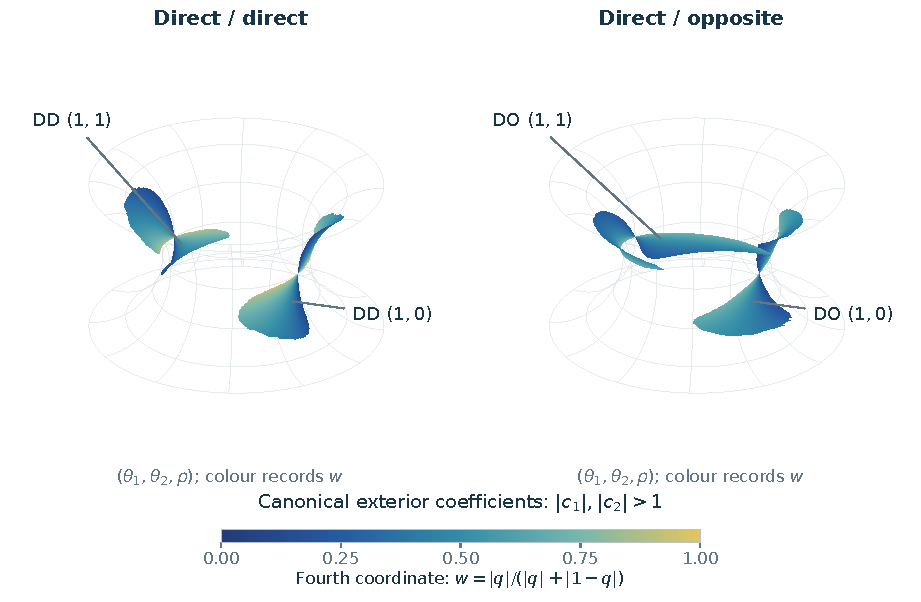
\includegraphics[width=\textwidth]{figures/four_family_projection.pdf}
\caption{Four selected stable slices placed in the four-dimensional
atlas by exterior coefficients $|c_1|,|c_2|>1$ and projected using
\eqref{eq:zipper-three-dimensional-projection}. DD and DO occupy
separate orientation charts. Colour records the fourth coordinate
$w$; the visible sheets consist of certified stable parameter cells.
The wireframe is the outer reference $\rho=2$. Position alone omits
$w$, and the imposed toroidal opening has no implication for the
topology of the connectedness locus. The canonical DO phase rotation
is included as in~\eqref{eq:four-exterior-surfaces}.}
\label{fig:zipper-stable-atlas}
\end{figure}

\begin{figure}[p]
\centering
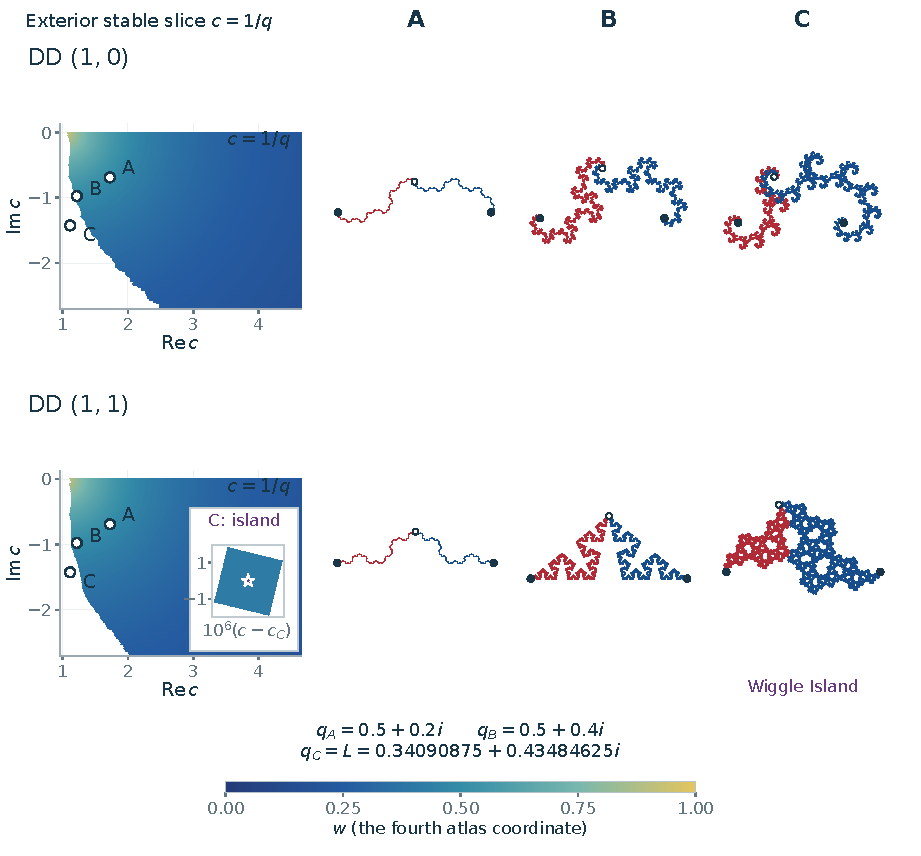
\includegraphics[width=\textwidth]{figures/four_family_DD.pdf}
\caption{DD$(1,0)$ and DD$(1,1)$: certified stable inner covers in the
unsigned endpoint coordinate $c=1/q$, linked to the three common
curve probes~\eqref{eq:three-shared-zipper-probes}. The corresponding
canonical exterior coordinates are $c_1=-c$ and
$c_2=(-1)^{e_2}c/(c-1)$. The DD$(0,1)$ reflection is represented
by DD$(1,0)$. Red and blue distinguish the first-level curve pieces;
they are not membership labels. The tiny certified DD$(1,1)$
neighbourhood of $L$ is shown separately from the common-scale cover.
The curve approximations and their error bounds are recorded in
Appendix~\ref{app:zipper-computation}.}
\label{fig:zipper-dd-gallery}
\end{figure}

\begin{figure}[p]
\centering
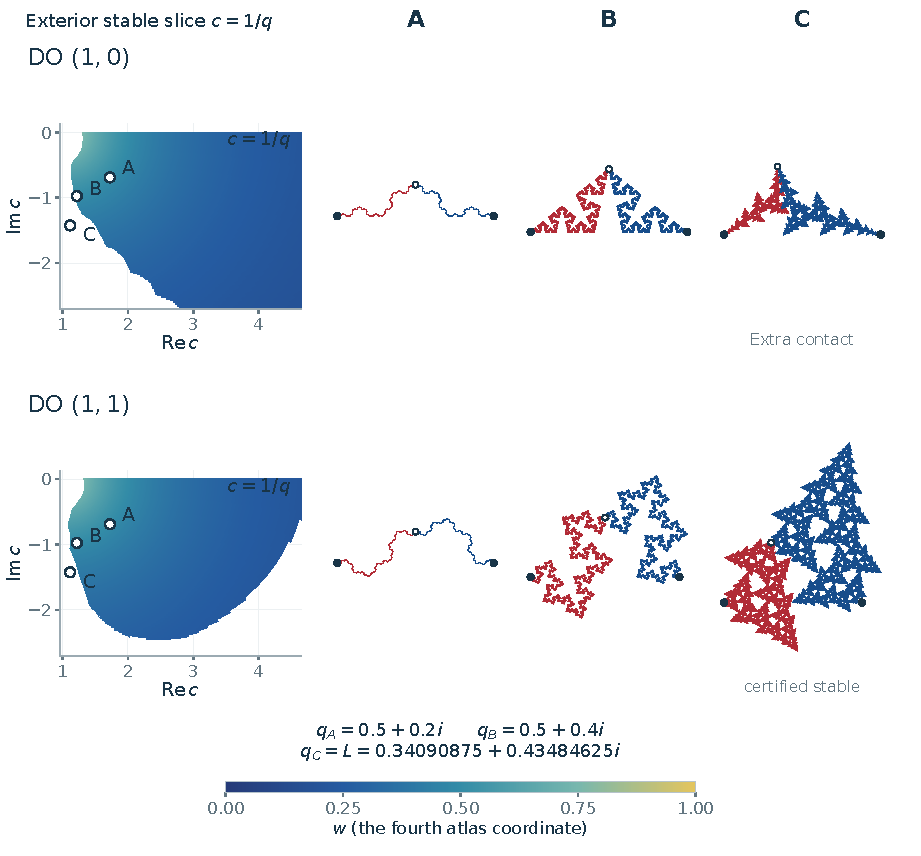
\includegraphics[width=\textwidth]{figures/four_family_DO.pdf}
\caption{DO$(1,0)$ and DO$(1,1)$ at the same exterior slice coordinates
and curve probes as Figure~\ref{fig:zipper-dd-gallery}. The opposite
map contributes the phase factor $N/\overline N$ in the canonical
exterior coefficient $c_2$. The painted slice regions certify stable
parameters. The common probe $q_C=L$ produces an additional
identification for DO$(1,0)$ and an embedded curve for DO$(1,1)$;
these conclusions come from certificates, independently of the
finite curve drawings.}
\label{fig:zipper-do-gallery}
\end{figure}



\section{Finite computation and what its output proves}
\label{sec:core-computation}

Let $r=\max\{|a|,|b|\}$ and $R=(1-r)^{-1}$. The closed disk
$B=\overline{D}(0,R)$ satisfies $S_1B\cup S_2B\subseteq B$.
Put $K_n=\bigcup_{|u|=n}S_uB$. These are nested compact outer
approximations of $K$, with Hausdorff error at most $2Rr^n$.

\begin{proposition}[Finite disconnection certificates]
\label{prop:finite-exclusion}
The attractor is disconnected if and only if some $n$ satisfies
$S_1K_n\cap S_2K_n=\varnothing$. Each such assertion reduces to
finitely many strict disk-separation inequalities. A parameter
that survives these tests to a finite depth has not thereby been
proved connected.
\end{proposition}
\begin{proof}
The sets $S_1K_n\cap S_2K_n$ are nested compact sets, and their
intersection is $S_1K\cap S_2K$. If every one is nonempty, compactness
gives a point in their intersection. Otherwise the empty stage
certifies disjoint first pieces. Each cylinder image of $B$ is a
disk, including for opposite similarities; the finite union
intersection is empty exactly when all cross-pairs of disks are
disjoint. The binary contact criterion completes the proof.
\end{proof}

Outward-rounded interval or ball arithmetic can turn strict
separation inequalities into validated certificates. Finite
survival is an outer approximation and should be labelled
``not excluded at depth $n$''. Positive certificates can instead
come from a proved sufficient region such as
\eqref{eq:modulus-bounds}, a verified zipper relation, or exact
address contacts forming a connected first-piece graph.

\begin{lemma}[Persistence of a positive contact gap]
\label{lem:contact-gap-persistence}
Fix the plane orientations and let the two coefficient pairs $\lambda$ and
$\mu$ have contraction ratios at most $\bar q<1$. Put
$\eta=\max_j|\lambda_j-\mu_j|$. For the corresponding attractors and
first-piece distances,
\[
 d_H(K_\lambda,K_\mu)\leq\frac{\eta}{(1-\bar q)^2},\qquad
 |\delta(\lambda)-\delta(\mu)|\leq\frac{2\eta}{(1-\bar q)^2}.
\]
If $\delta(\lambda)\ge d_0>0$ and
$\eta\le d_0(1-\bar q)^2/4$, then $K_\mu$ is disconnected with first-piece
gap at least $d_0/2$.
\end{lemma}
\begin{proof}
Both attractors lie in the disk of radius $R=(1-\bar q)^{-1}$. Their
Hutchinson operators differ by at most $\eta R$ on every compact subset of
this disk. The contraction estimate therefore gives
\[
 d_H(K_\lambda,K_\mu)
 \leq\bar q\,d_H(K_\lambda,K_\mu)+\eta R,
\]
which proves the first bound. Either corresponding first-level piece is
displaced by at most
$\bar q\,d_H(K_\lambda,K_\mu)+\eta R\le\eta/(1-\bar q)^2$.
The distance between two compact sets changes by at most the sum of their
Hausdorff displacements, proving the second bound and its consequence.
\end{proof}

For a rational centre with a rational verified gap bound $d_0>0$, let $q<1$ be a rational outward
bound for both multiplier moduli and put $\bar q=(1+q)/2$. The radius
\begin{equation}\label{eq:rational-neighbourhood-radius}
 \eta_0=\min\left\{\frac{1-q}{2},\,
           \frac{d_0(1-\bar q)^2}{4},\,
           \frac12\min_j\max(|\Re\lambda_j|,|\Im\lambda_j|)\right\}
\end{equation}
defines a closed product of complex disks
$|\mu_j-\lambda_j|\le\eta_0$ lying in the punctured contraction bidisk.
Every parameter in this product has gap at least $d_0/2$. Its interior is
an explicit open disconnected region in four real dimensions.


An address chosen by a finite search is a witness selected by that
algorithm and its tie-breaking rule. A colour change between such
addresses does not, without further proof, establish a topological
stratum, an entropy invariant or a smooth frontier branch. Boundary
meshes should therefore record the depth, enclosure bound, decision
status and witness-selection rule. Radial scans must retain all
detected transition intervals unless a one-transition theorem has
been established for the region being rendered.

% Portable section for the revised paper. Requires amsmath, amssymb, hyperref.
% Inspected source snapshot: complextrees.com/4D/, accessed 18 September 2026.
\section{From symbolic contact to a navigable atlas}
\label{sec:explorer-methods}

The companion \emph{Connectedness Atlas} implements a common passage from a
parameter to its maps, symbolic cylinders, contact data and planar geometry.
The parameter inspector and exported specimen records retain the four coordinates
$(\alpha,\gamma,\rho,w)$ and the orientation pair. Thus a point chosen in a
three-dimensional display can be returned to an explicit planar system. The
implementation and mathematical conventions are available at
\url{https://complextrees.com/4D/}; the source snapshot discussed here was
inspected on 18 September 2026.

\subsection{Paired words and their enclosures}
Use $\lambda_-=a$, $\lambda_+=b$ and the signs $\kappa_j$ of Section~\ref{sec:core-normalization}. An accumulated cylinder map is stored as
\[
F_u(z)=t_u+L_u J_{\kappa_u}z.
\]
Appending a letter $j$ on the right gives the recurrence
\begin{equation}\label{eq:atlas-prefix-recurrence}
 t_{uj}=t_u+L_u J_{\kappa_u}(t_j),\qquad
 L_{uj}=L_u J_{\kappa_u}(\lambda_j),\qquad
 \kappa_{uj}=\kappa_u\kappa_j,
\end{equation}
where signs are multiplied. The implementation stores them as parity bits. This outermost-first convention makes
the first address symbol identify an actual first-level piece, including for
orientation-reversing maps.

The marked difference for the normalized system is
\[
D_p=\lambda_- J_{\kappa_-}(K_p)-\lambda_+ J_{\kappa_+}(K_p),
\qquad K_p\text{ is connected}\ \Longleftrightarrow\ 2\in D_p.
\]
An unequal-multiplier or reversing system is evaluated through two accumulated
maps and two parity bits. On the common direct-multiplier slice this reduces to
the usual homogeneous difference construction. Equal contraction ratios alone
do not make that reduction valid.

Let $q=\max(|\lambda_-|,|\lambda_+|)<1$ and $R=(1-q)^{-1}$.
The invariant disk $\overline B(0,R)$ supplies each word with the enclosure
\[
F_u(K_p)\subseteq \overline B(t_u,R|L_u|).
\]
A cross-prefix pair $(u,v)$ can therefore be discarded when
$|t_u-t_v|>R(|L_u|+|L_v|)$. The implementation develops the remaining pairs
in four children. Complete exhaustion gives finite separation; otherwise the
output retains a surviving frontier or the reason that a work limit stopped
the search. The browser uses this procedure to locate parameters worth refining.
For exact rational coefficients, a separate implementation replaces modulus
estimates by rational outward bounds and compares squared distances exactly.

The resulting proof object is a finite prefix antichain covering every infinite
cross-prefix address pair. Its independent checker reconstructs word maps with
rational real $2\times2$ matrices, verifies cover completeness and checks every
strict separation inequality. A successful record also supplies a positive
contact gap and an explicit product of complex parameter disks on which that
gap remains positive. This provides a constructive route from an atlas sample
to an open disconnected region in four real dimensions. It does not require
the visualization to decide membership.

\subsection{Radial surveys and three-dimensional navigation}
At a fixed weight and orientation, the survey samples the angular variables and
searches the radial interval
\[
 2\sqrt{w^2+(1-w)^2}\leq\rho\leq2.
\]
The inner endpoint comes from the closed square-sum connectedness criterion;
the outer endpoint comes from the sum-of-ratios obstruction. The current
three-orientation explorer samples an entire radial interval, brackets each
detected survival--exclusion or exclusion--survival transition, and refines
those brackets. It records re-entry bands and unresolved searches. The visible
surface uses the outermost detected finite-survival sheet. A narrow band may
fall between samples, so the recorded transition list remains part of the data.

The detailed direct--direct laboratory at \url{https://complextrees.com/4D/lab/}
contains $13\times41\times81=43\,173$ sampled rays: thirteen weights from
$0.35$ to $0.65$, with $41$ values of $\alpha$ and $81$ values of $\gamma$.
It retains two search depths, the first and outer exits, band counts and
cross-depth discrepancies. A rectangular chart displays the original stored
samples, while angular cosine interpolation and a cubic spline in weight
supply the smooth three-dimensional display. Selecting or exporting a stored
cell retains its original data. The display mesh and the radial survey therefore
have separate resolutions.

Paired letters are encoded by four symbols. The atlas can colour a parameter by
a selected surviving finite word pair or compare complete retained prefix data.
Such fields organize numerical experiments and expose changes that can be
examined through the address-equivalence relation. A constant finite label is
not used as the definition of stability. Likewise, a toroidal embedding is a
coordinate display; its imposed central hole does not classify the topology of
the connectedness locus.

\subsection{Exact families as navigable subsets}
The family registry places exact parameterized systems in the same coordinates
as the free atlas. In particular, it implements the twelve marked binary
zipper presentations obtained from three unordered planar orientation types
and four traversal signatures. Each uses the strict lens
$|z|<1$, $|1-z|<1$, evaluates its endpoint maps, and normalizes the resulting
pair. The traversal bits and the planar parity remain separate fields.
These are twelve marked presentations; no assertion that their images are
pairwise disjoint or that they classify every connected binary attractor is
needed. The comparative figures select DD$(1,0)$, DD$(1,1)$, DO$(1,0)$
and DO$(1,1)$. Their coefficient-phase projection is defined in
Section~\ref{sec:exterior-zipper-atlas}; it preserves the canonical
normalization of the registry, including the phase rotation of the
opposite map. It is a separate figure construction from the earlier
$(\alpha,\gamma)$ display of the six-specimen survey below.

The same normalization accepts the binary complex-tree families defined by
explicit eventually periodic address relations. Their records carry the raw
tree maps, the contact words, the cleared relation and the resulting normalized
parameter. The reader can therefore move between the original tree alphabet,
an algebraic contact family, a marked zipper when available, and the ambient
four-dimensional chart without changing conventions silently.

\subsection{Finite geometry, hulls and empirical difference images}
The planar renderer enumerates all words at the reported depth and carries their
first-level piece and parity. It computes in binary64 and draws binary32 vertex
buffers using a worker and WebGL~2, with a Canvas fallback. Geometry budgets
choose the actual depth; the export records that depth and the number of
prefixes drawn. Camera movement and a finer raster do not change the underlying
word set.

In exact arithmetic, with $Z_N=\{F_u(0):|u|=N\}$,
\begin{equation}\label{eq:atlas-finite-geometry-error}
 d_H(K_p,Z_N)\leq Rq^N,
 \qquad
 d_H(D_p,D_{p,N}^{\rm ctr})\leq
 (|\lambda_-|+|\lambda_+|)Rq^N,
\end{equation}
where $D_{p,N}^{\rm ctr}$ uses the two transformed copies of $Z_N$. Convexification is
nonexpansive for Hausdorff distance, so these bounds also compare the filled
finite convex hulls with the corresponding limiting convex hulls. The drawn
outlines are computed from finite floating-point centres; the analytic tail
bound does not by itself enclose every floating-point error.

The six-sample study at \url{https://complextrees.com/4D/atlas/} uses
$N=22$, hence $2^{22}$ addressed centres per attractor. Its difference images
retain word multiplicities by taking a histogram cross-correlation of the two
transformed word clouds. This represents $2^{44}$ ordered pairs without
enumerating every pair explicitly. The quantity displayed is the probability
per unit area for independent uniform finite words on the specified lattice.
A shared logarithmic opacity scale permits comparison across specimens.
For nearest-lattice rounding with spacing $h$, rounding the two clouds before
subtraction adds at most $\sqrt2 h$ of geometric displacement, in addition to
the finite-tail and arithmetic errors. This finite distribution is not assumed
to be a density of a limiting measure.


\subsection{Six linked parameter specimens}
Figures~\ref{fig:atlas-overview} and~\ref{fig:atlas-specimens} provide a linked
view of the parameter atlas and the planar sets it describes. The six samples
share $w=1/2$ and direct orientations, but generally have different complex
multipliers. Table~\ref{tab:six-specimens} records the phase representatives
and radial values used by the figures. In this display the angular embedding is
\[
 (\alpha,\gamma,\rho)\longmapsto
 \bigl((4+\rho\cos\alpha)\cos\gamma,
       \rho\sin\alpha,(4+\rho\cos\alpha)\sin\gamma\bigr).
\]
It is a visualization of a phase-chart representative, with the seam metadata
retained; it is not asserted to be a globally injective embedding of the
phase-lattice quotient. A specimen links that display position to two planar
objects: $K_p$, with its first-level decomposition, and $D_p$, with the target
point $2$. In this way the same parameter can be examined through ambient
position, geometry and finite symbolic contact information.

\begin{figure}[tbp]
\centering
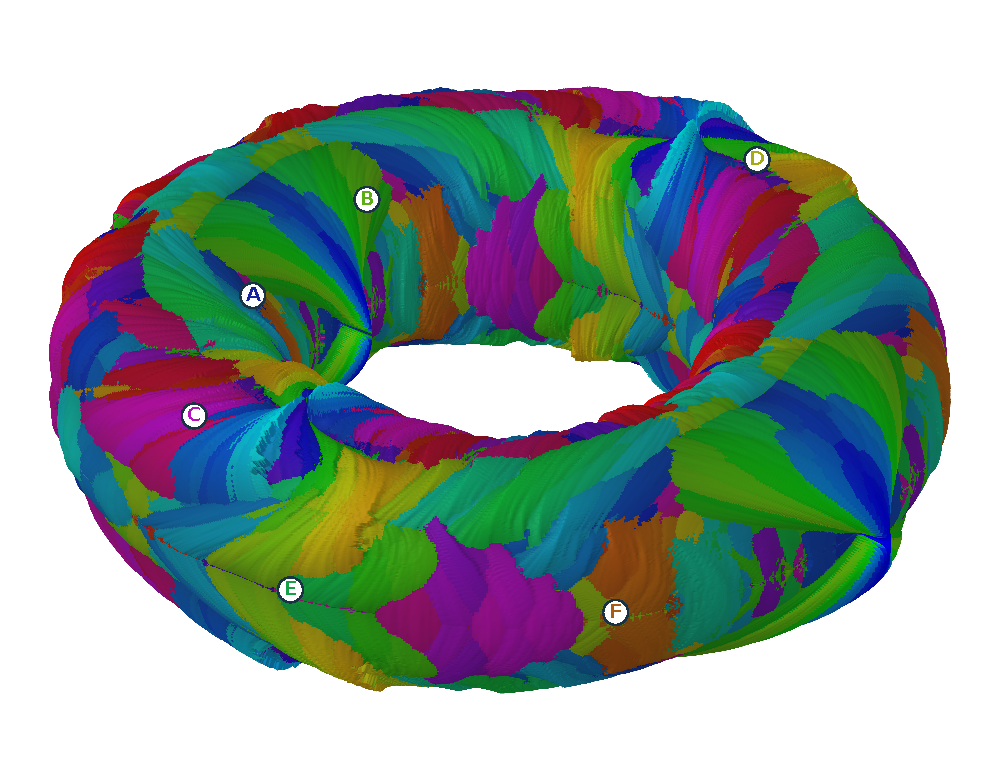
\includegraphics[width=\linewidth]{figures/Atlas_4D_Paper_Atlas.pdf}
\caption{Equal-contraction DD parameter atlas with specimens A--F. The angular
view displays the finite numerical study underlying the companion explorer.
Colours record selected finite pair-address codes. The central hole belongs
to the coordinate display. Parameters are given in
Table~\ref{tab:six-specimens}, with planar sets in
Figure~\ref{fig:atlas-specimens}.}
\label{fig:atlas-overview}
\end{figure}

\begin{figure}[tbp]
\centering
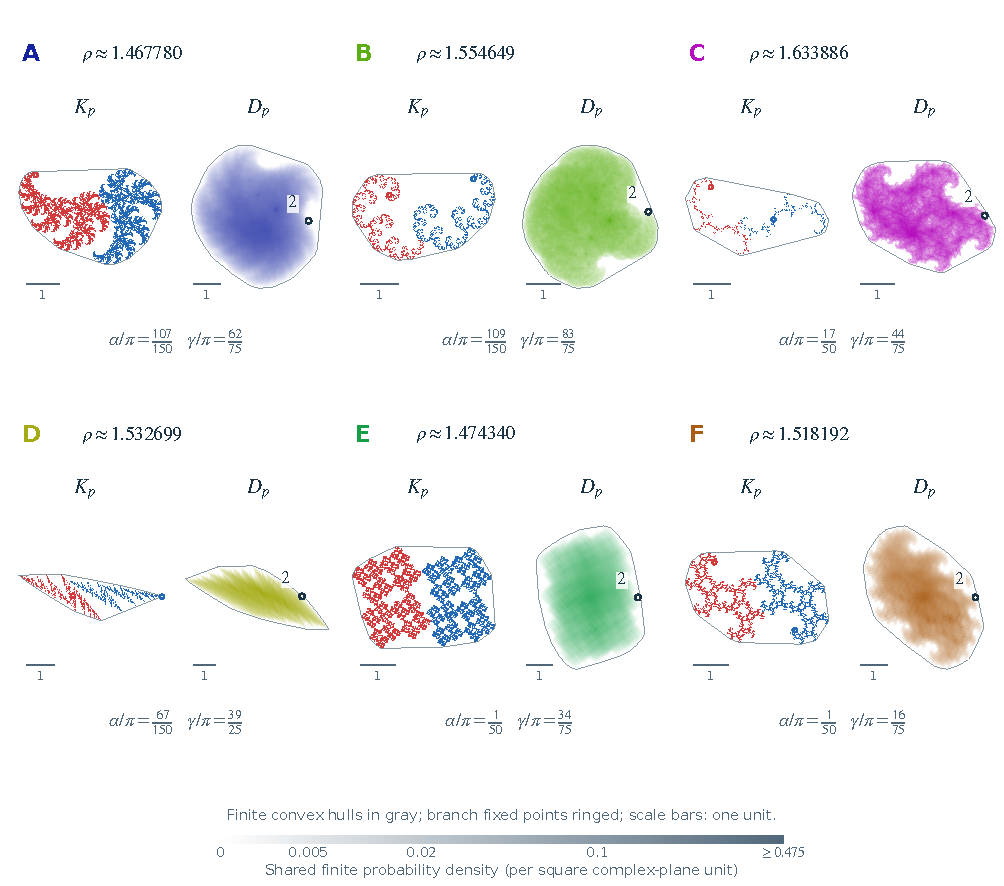
\includegraphics[width=\linewidth]{figures/Atlas_4D_Paper_Specimens.pdf}
\caption{The six linked specimens. Red and blue show first-level pieces of
$K_p$; $D_p=aK_p-bK_p$ uses the corresponding atlas hue and a shared finite
probability-density scale. Every attractor uses all length-22 addressed
centres. Gray outlines are finite convex hulls, rings in $K_p$ mark branch
fixed points, and the ring in $D_p$ marks $2$. Scale bars have length one;
panels are fitted independently. The images do not certify exact contact.}
\label{fig:atlas-specimens}
\end{figure}
\begin{table}[tbp]
\centering\small
\begin{tabular}{@{}crrrrr@{}}
\toprule
Sample & $\alpha/\pi$ & $\gamma/\pi$ & $\rho$ & $Rq^{22}$ & $2qRq^{22}$\\
\midrule
A & $\frac{107}{150}$ & $\frac{62}{75}$ & 1.4677798748 & $6.76\mathbin{\times}10^{-4}$ & $9.21\mathbin{\times}10^{-4}$ \\
B & $\frac{109}{150}$ & $\frac{83}{75}$ & 1.5546487570 & $1.70\mathbin{\times}10^{-4}$ & $2.19\mathbin{\times}10^{-4}$ \\
C & $\frac{17}{50}$ & $\frac{44}{75}$ & 1.6338859797 & $5.25\mathbin{\times}10^{-5}$ & $6.43\mathbin{\times}10^{-5}$ \\
D & $\frac{67}{150}$ & $\frac{39}{25}$ & 1.5326993465 & $2.39\mathbin{\times}10^{-4}$ & $3.12\mathbin{\times}10^{-4}$ \\
E & $\frac{1}{50}$ & $\frac{34}{75}$ & 1.4743398428 & $6.07\mathbin{\times}10^{-4}$ & $8.24\mathbin{\times}10^{-4}$ \\
F & $\frac{1}{50}$ & $\frac{16}{75}$ & 1.5181920528 & $3.00\mathbin{\times}10^{-4}$ & $3.96\mathbin{\times}10^{-4}$ \\
\bottomrule
\end{tabular}
\caption{Parameters of the six equal-contraction DD specimens ($w=1/2$),
with $q=1/\rho$. Radial values are rounded here; the full numerical record
is retained in the source. The last columns are analytic tail estimates
in exact arithmetic, excluding floating-point and density-grid errors.}
\label{tab:six-specimens}
\end{table}

\subsection{Reproducible states and figures}
The mathematical record consists of coefficients, orientations, word convention,
sampled grids, budgets, retained evidence and arithmetic. The figure record adds
the camera, projection, raster, display mesh, colour map and finite geometric
depth. The explorer exports these independently of the image through JSON
records and embeds parameter metadata in PNG files. The detailed laboratory
also provides raw slice CSV and validated session records. These records allow a
figure to be reproduced while preserving the distinction between a mathematical
parameter, the computation performed there and its visual presentation.

\section{Contact geometry and further directions}
\label{sec:discussion}

The atlas connects three levels of description. A parameter determines a compact
attractor; its coding map records which symbolic points are identified; and its
position within a prescribed contact family determines which of those
identifications are forced. The exact examples show why these levels are useful
together. The quarter-turn attractor has four different semilinear presentations
with the same first-level pieces, while their agreement is established by
explicit recodings. At the critical rectangle its first-level intersection is a
segment, with different address multiplicities along that segment. On a whole marked binary zipper
surface, by contrast, the stable set consists precisely of the embedded
canonical curves. A single geometric contact label cannot describe all of these
situations.

The triangle family makes the universal radial bounds concrete. Its elementary
altitude dissection belongs to the classical geometry of self-similar tiles;
related two-piece planar tiles are studied in~\cite{NgaiSirventVeermanWang2000}.
Here the explicit normalization places such a family on the connectedness
boundary at every contraction weight, and the separated perturbation proves
sharpness in the full opposite--opposite chart. The opposite diagonal gives a
second exact model: its circle and real antennae produce a discontinuous radial
ceiling. Thus a smooth displayed sheet can be informative while missing genuine
features of the parameter boundary.

Several precise questions follow from these constructions. Near a critical
triangle or rectangle, which directions in the full coefficient space preserve
contact, produce separation, or create positive-area overlap? The formulas for
the exact families provide base parameters at which to study this local change.
For a fixed eventually periodic pair, the contact equation is algebraic; one
can ask when its regular branches organize nearby fixed-address fibres and when
additional contact pairs change their local structure. These questions concern
both the geometry of a fibre and the way fibres intersect.

The stable-set construction supplies a common language for the complex-tree
families developed since~\cite{Espigule2013,Espigule2018,Espigule2019a} and for
marked zippers. Calegari's island theorem gives a disconnected embedded locus
on one zipper surface~\cite{Calegari2026}. It is natural to seek other prescribed
contact families with disconnected stable sets, and to compare their forced
quotients and excess-contact fibres. Passing from a slice to a larger family
changes the forced relation, so any persistence statement should specify the
family and coding relation under consideration. The exterior-coordinate
comparison makes this distinction visible: the four selected stable slices
are subsets of their marked zipper surfaces in the four-dimensional atlas,
and colour retains their contraction weight after projection to three
dimensions. Intersections in the projection can therefore arise from
different weights; they do not themselves identify systems or contacts.

The companion atlas makes these questions accessible as reproducible
experiments. Finite radial surveys suggest regions to investigate; exact
contact relations provide positive examples; complete prefix covers and the
contact-gap estimate provide open sets of certified separation. The next
computational step is to adaptively refine those records around specified
contact fibres and their intersections. This extends the atlas through explicit
mathematical questions and checkable parameter data, while the visualization
continues to support immediate movement between parameters and attractors.

\appendix
\section{Reproducibility and exact computation records}
\label{app:reproducibility}

The companion reproducibility archive separates the mathematical record from the
current browser interface. It contains the figure-generation records, exact
certificates, and public assets from which the scientific plates are recomposed;
the arXiv source retains the files required to compile this article and the
small exact certificate suite used below. The study uses all length-22 addressed centres
for each attractor. Its preserved density rasters and atlas rendering are
recomposed without asserting that the global radial survey has been rerun.
The independent overlay script reconstructs each finite convex hull and checks
the multipliers, branch fixed points and analytic tail formulas against the
stored record. These are floating-point consistency checks.

The inspected companion snapshot is dated 18 September 2026. A source manifest
records the original URL, byte size and SHA--256 digest of the inspected
modules. The principal mathematical implementations are the family registry,
the semilinear prefix renderer and the radial worker. The DD laboratory's
$43\,173$-ray data record reassembles to 5,913,659 bytes, with SHA--256 digest
\begin{center}\footnotesize\ttfamily
5d833a368c0a43405d512ecd0e5a7a53c\linebreak
ddd19a019142b9ed9f6f05e94a64af9.
\end{center}
The manifest distinguishes this frozen record from later changes to the public
interface. The detailed laboratory's source and data harness passed 73 checks;
its grid, picking and session harness passed 3,381 enumerated checks. These
results concern the inspected code and data, and are not frame-rate measurements.

\subsection{A small exact benchmark suite}
The reference computation uses rational complex coefficients and exact rational
comparisons. Let $r_*<1$ be a rational upper bound for both contraction ratios,
verified by comparing their squared moduli with $r_*^2$, and put
$R_*=(1-r_*)^{-1}$. For equal-length words $u,v$ of length $n$, with opposite
first symbols, write $c_u=S_u(0)$ and $c_v=S_v(0)$. The pair is excluded only if
\begin{equation}\label{eq:exact-disk-exclusion}
|c_u-c_v|^2>(2r_*^nR_*)^2.
\end{equation}
The two cylinder images lie in the corresponding enclosing disks, so this
strict inequality is a sufficient separation certificate.

The search starts with the first-piece pair, discards excluded pairs, and
otherwise branches over all four choices of appended letters. Complete finite
exhaustion certifies disconnection. A depth or pair limit leaves an unresolved
frontier. The output records all excluded and unresolved leaves, together with
the exact squared distances and bounds. The independent verifier reconstructs
cylinder centres by evaluating the letters from right to left and checks both
the inequalities and the complete four-child covering tree. It imports no
producer code.

Table~\ref{tab:exact-benchmarks} gives the completed benchmark runs. The depth
limit was 8 and the pair limit 20,000. Each row applies separately to every
orientation type listed. All resulting records passed the standalone verifier.
\begin{table}[htbp]
\centering\small
\begin{tabular}{@{}llrrrl@{}}
\toprule
Coefficients $a=b$ & Orientation types & Depth & Tests & Excluded & Output\\
\midrule
$1/4$ & $(+,+)$ & 1 & 1 & 1 & Disconnected\\
$2i/3$ & $(+,+),(+,-),(-,-)$ & 6 & 69 & 52 & Disconnected\\
$1/2$ & $(+,+),(+,-),(-,-)$ & 8 & 29 & 21 & Unresolved\\
\bottomrule
\end{tabular}
\caption{Exact rational exclusion experiments. Depth counts the full cylinder
word length, including its first symbol. Each $2i/3$ run has 17 split pairs and
no surviving frontier; each $1/2$ run has seven split pairs and one surviving
frontier pair. ``Excluded'' counts leaf pairs, not parameters.}
\label{tab:exact-benchmarks}
\end{table}

For $a=b=1/2$, the elementary interval identity
$S_1([-2,2])=[-2,0]$ and $S_2([-2,2])=[0,2]$ proves that the attractor is
$[-2,2]$ in each orientation type. Thus the unresolved search output is
consistent with a separate exact connectedness proof. The experiment checks
the one-sided logic of exclusion; it does not implement a global classification
of the atlas.

The \texttt{computation/} directory contains the producer
\path{exact_exclusion.py} and the independent verifier
\path{verify_certificate.py}. The seven JSON records and their
summary are in \path{computation/certificates/}. These small examples establish
a reproducible starting point for the computational method. Larger frontier
claims require their own complete certificates or a proved positive criterion.


\subsection{Parameter-neighbourhood proof objects}
The companion's version~2.0.0 rational producer and independent checker are
included under \path{computation/neighbourhood/}. Their exact inputs specify the
two multipliers as decimal or fraction strings and the two orientation bits.
The producer uses individual rational outward bounds for word contractions;
the checker reconstructs the affine maps with rational real matrices and checks
the complete prefix cover. It then verifies the positive-gap neighbourhood from
Lemma~\ref{lem:contact-gap-persistence}. Its 23-test suite includes independent
exact-family benchmarks and rejection of incomplete or altered proof objects.

For example, the opposite--opposite parameter
$a=b=3(1+i)/8$ is certified by four cover leaves of word length two.
The exact checked gap exceeds $13/50$ and the parameter radius exceeds
$1/300$. Consequently the complete product
\[
 |a'-3(1+i)/8|\le1/300,\qquad |b'-3(1+i)/8|\le1/300
\]
has disconnected attractors with first-piece gap at least $13/100$.
The companion archive retains both the proof object and the independently checked record.

The two producers use the same mathematical separation criterion but different
schemas and enclosure choices. Each proof object identifies its producer and
is checked with the matching standalone checker. Rounding a trigonometric
coefficient supplies an exact rational centre different from the intended
trigonometric parameter; transferring a neighbourhood claim to the latter
requires rigorous containment. The companion archive's README gives the complete commands for the manuscript, figures and exact checks.


\subsection{The four-family exterior comparison}
\label{app:zipper-computation}
Figures~\ref{fig:zipper-stable-atlas}--\ref{fig:zipper-do-gallery}
transform positive certificates from a $512\times256$ dyadic grid
on $[0,1]\times[0,1/2]$ in the endpoint $q$ plane. Each cell has side
$1/512$. The original endpoint-return calculation used a budget of
$12\,000$ cylinder-pair visits and maximum word length 40. Success
means that \emph{every parameter} in the closed cell is embedded.
A computation that does not finish gives no membership conclusion.
The selected covers are DD10, DD11, DO10 and DO11. The DD10 record
also includes cells obtained from DD01 by the exact reflected
symmetry $q\mapsto1-\overline q$; the duplicate family is omitted
from the figures. Complex conjugation supplies the reflected
lower-half cover in the three-dimensional placement. The unpainted
background carries no membership label. Exact OO stable-disk
classifications are proved in the text and are not drawn in this
four-family comparison.

The planar coordinate is $c=1/q$; the three-dimensional position
uses the canonical coefficients of
Proposition~\ref{prop:four-exterior-surfaces}, not just the endpoint
multipliers. Both transformations are applied to the saved positive
cells. The exterior panels retain the full $512\times256$ positive
mask, clipped to $[0.96,4.65]\times[-2.70,0.13]$ in the $c$ plane.
The unbounded tail near $q=0$ lies beyond this window. For the
three-dimensional mesh, a $2\times2$ block is included only when
all four original closed cells are certified; this thinning can
omit positive cells but does not bridge uncertified gaps. The
figure mesh approximates the curved images of those blocks. Exact
cell coordinates and membership certificates are retained
separately. The colour coordinate is $w$. The projection and image-generation
records are retained in the companion archive under \path{figure_sources/four_families/}.

The interval implementation uses IEEE binary64 arithmetic with outward
\texttt{nextafter} bounds, including contraction norms, invariant radii,
cylinder centres and squared separation. Its recorded build uses GCC
13.3.0, with fast-math and fused contraction disabled. Gradual underflow
and correctly rounded elementary operations, including square root, are
assumed. An independent integer-polynomial checker verifies all fourteen
common-return identities. A separate compilation reproduced the saved
island-rectangle calculation; this is a replay of the same interval
implementation, rather than a second numerical algorithm. The complete commands, exact parsed bounds, per-cell outcomes and file hashes are retained in the companion archive under
\path{figure_sources/zippers/zipper_stability_run_manifest.json}.

For the curve examples, iterate the zipper operator from the identity
map on $[0,1]$ with equal partition intervals. Write
$r=\max\{|q|,|1-q|\}$. The first polygon differs from the identity by at
most $|q-1/2|$, so the depth-$n$ polygon $\zeta_n$ satisfies
\[
 \|\zeta-\zeta_n\|_\infty
 \le \frac{r^n|q-1/2|}{1-r}.
\]
The figures use the three shared probes in
\eqref{eq:three-shared-zipper-probes}. At $q_A$ and $q_B$, depth 20
gives $1\,048\,577$ vertices, with respective uniform bounds
$1.824\times10^{-6}$ and $1.493\times10^{-4}$.

At $q_C$ the two contraction ratios differ substantially, so an
adaptive prefix partition gives a better display for the same
number of segments. First bound
$E=\|\zeta-\operatorname{id}\|_\infty$ using the exact depth-14
polygon and the tail estimate above: the maximum norm of its
difference from the identity occurs at a polygon vertex. On a
source cylinder with $m$ occurrences of the first symbol and $n$
of the second,
the endpoint chord then has parametrized error at most
$|q_C|^m|1-q_C|^n E$. Subdivide until a rational upper bound for
this product is at most $1/2000$. The leaves form an exact
partition of $[0,1]$, and all four curves have uniform error
strictly less than $5\times10^{-4}$ in exact arithmetic.
The vertex counts and source depths are
\begin{center}
\begin{tabular}{lrr}
Family&Vertices&Source depths\\\hline
DD10&$724\,014$&13--31\\
DD11&$473\,538$&12--30\\
DO10&$462\,020$&12--30\\
DO11&$1\,692\,525$&14--34
\end{tabular}
\end{center}
The plotted coordinates are evaluated in binary64; the analytic
error bounds exclude this final floating-point evaluation and
rasterization. Exact stopping decisions, source-partition checks
and the resulting arrays are retained in the companion archive under
\path{figure_sources/four_families/specimen_checks/}.
Drawing a polygon without visible crossings is not used as a
positive certificate. Ten
positive interval records certify $q_A,q_B$ in all four families
and $q_C$ in DD11 and DO11. Each test applies to a closed dyadic
box of side $2^{-34}$ containing the stated exact rational
parameter, with a budget of $2\,000\,000$ cylinder-pair visits
and maximum word length 100.

An additional exact calculation proves that the DO10 canonical
curve at $q_C$ is nonembedded. With letters $0,1$ denoting the
first and second maps, respectively, take words
$u=00011100$ and $v=101101111111$. Their closed parameter intervals
are $[33/128,67/256]$ and $[2303/4096,9/16]$, which are disjoint.
For $G(s,t)=F_u\zeta(s)-F_v\zeta(t)$ on $[0,1]^2$, a cover by
46 cylinder enclosures keeps its boundary away from zero and
certifies boundary degree $-1$. Nonzero degree supplies a zero
of $G$, hence an identification between the two disjoint
parameter intervals. The coefficient arithmetic and strict
disk-separation comparisons are rational; an independent checker
reconstructs the enclosures and computes winding using a
different ray. The proof object and replay record accompany the positive probe records in the companion archive under
\path{figure_sources/four_families/specimen_checks/}. No conclusion
about DD10 at $q_C$ follows from its capped positive test.

Finally, the small DD11 square
\[
\begin{split}
0.3409082591533661&\le\Re q\le0.3409092128276825,\\
0.4348457604646683&\le\Im q\le0.4348467141389847
\end{split}
\]
uses the exact dyadic endpoints recorded in hexadecimal in the run
manifest; the displayed decimals are their round-trip representations.
All $64^2=4096$ cells of side $2^{-26}$ pass, with a budget of
$150\,000$ visits per cell and maximum word length 64. This proves
embeddedness throughout the square, which contains Calegari's rational
island parameter $L=0.34090875+0.43484625i$. Its membership in a component
separate from the real interval follows from the cited island theorem,
not from this local calculation. The whole square has side $2^{-20}$;
it is too small to see in the common-scale atlas and is not intended
as a depiction of the island boundary.


\section*{Funding}
This work was supported by the Spanish Ministerio de Ciencia, Innovaci\'on y
Universidades through project PID2023-146424NB-I00.

\section*{Data and code}
The companion explorer is available at \url{https://complextrees.com/4D/}.
The companion repository at \url{https://github.com/espigule/ComplexTrees}
contains the figure-generation scripts, exact parameter records and finite
disconnection certificates used in this article, together with an independent
verifier. Section~\ref{sec:explorer-methods} gives the
computational conventions, and the accompanying source record identifies the
inspected explorer version and figure assets. All numerical images are
labelled by their approximation method; the exact phase diagrams follow from
the proofs in the text.

{\small\raggedright\setlength{\parskip}{0pt}\begin{thebibliography}{99}
\setlength{\itemsep}{3pt}
\bibitem{Hutchinson1981}
J.~E. Hutchinson, \emph{Fractals and self similarity},
Indiana Univ. Math. J. \textbf{30} (1981), no.~5, 713--747.
\href{https://doi.org/10.1512/iumj.1981.30.30055}{doi:10.1512/iumj.1981.30.30055}.

\bibitem{Hata1985}
M. Hata, \emph{On the structure of self-similar sets},
Japan J. Appl. Math. \textbf{2} (1985), 381--414.
\href{https://doi.org/10.1007/BF03167083}{doi:10.1007/BF03167083}.

\bibitem{BarnsleyHarrington1985}
M.~F. Barnsley and A.~N. Harrington,
\emph{A Mandelbrot set for pairs of linear maps},
Physica D \textbf{15} (1985), no.~3, 421--432.

\bibitem{Bandt2002}
C. Bandt, \emph{On the Mandelbrot set for pairs of linear maps},
Nonlinearity \textbf{15} (2002), no.~4, 1127--1147.

\bibitem{CalegariKochWalker2017}
D. Calegari, S. Koch and A. Walker,
\emph{Roots, Schottky semigroups, and a proof of Bandt's conjecture},
Ergodic Theory Dynam. Systems \textbf{37} (2017), no.~8, 2487--2555.

\bibitem{Aseev2003}
V. Aseev, A. Tetenov and A. Kravchenko,
\emph{On self-similar Jordan curves on the plane},
Siberian Math. J. \textbf{44} (2003), no.~3, 379--386.
\href{https://doi.org/10.1023/A:1023848327898}{doi:10.1023/A:1023848327898}.

\bibitem{RaoZhang2019}
H. Rao and S.-Q. Zhang,
\emph{Space-filling curves of self-similar sets (III): Skeletons},
arXiv:1804.10480, version~3, 2019.
\url{https://arxiv.org/abs/1804.10480v3}.

\bibitem{NgaiSirventVeermanWang2000}
S.-M. Ngai, V.~F. Sirvent, J.~J.~P. Veerman and Y. Wang,
\emph{On two-reptiles in the plane},
Geom. Dedicata \textbf{82} (2000), 325--344.

\bibitem{Espigule2013}
B. Espigul\'e Pons, \emph{Generalized self-contacting symmetric fractal trees},
Symmetry: Culture and Science \textbf{24} (2013), nos.~1--4, 320--338.
\href{https://journal-scs.symmetry.hu/content-pages/volume-24-numbers-1-4-pages-001-512-2013/}{Official issue record}.

\bibitem{Espigule2018}
B. Espigul\'e Pons,
\emph{Complex trees and their families of connected self-similar sets},
Master's thesis, Universitat de Barcelona, 28 June 2018.
\url{https://hdl.handle.net/2445/129385}.

\bibitem{Espigule2019a}
B. Espigul\'e,
\emph{Families of connected self-similar sets generated by complex trees},
arXiv:1902.11282, 2019.
\url{https://arxiv.org/abs/1902.11282v4}.

\bibitem{Espigule2019b}
B. Espigul\'e, \emph{A Family of Fern-like Ternary Complex Trees},
in Proceedings of Bridges 2019: Mathematics, Art, Music, Architecture,
Education, Culture, Tessellations Publishing, 2019, 147--154.
\url{https://archive.bridgesmathart.org/2019/bridges2019-147.html}.

\bibitem{Espigule2022Cornell}
B. Espigul\'e,
\emph{Families of Connected Self-similar Sets, 7th Fractals Conference,
June 7th 2022, Cornell University}, recorded lecture, 7 June 2022.
\url{https://www.youtube.com/watch?v=lpy3-VloR7s&t=1631s}.

\bibitem{Espigule2026Unilab}
B. Espigul\'e, \emph{La frontera secreta dels fractals}, UniLab26 workshop,
Universitat de Girona, 25 April 2026. Interactive materials for the
three four-dimensional connectedness families, publicly released 24 April 2026.
\url{https://complextrees.com/unilab26/}.

\bibitem{Espigule2026Thesis}
B. Espigul\'e Pons.
\emph{Collinear Fractals and Connectedness Loci: Topology, Finite Capture, and
Restricted Polynomial Roots}.
Doctoral thesis (submitted), Universitat de Girona, 2026.
Corrected circulation edition, 15 September 2026; deposited 9 September 2026.
\url{https://complextrees.com/research/thesis/}.

\bibitem{EspiguleJuherSaldana2024}
B. Espigul\'e, D. Juher and J. Salda\~na,
\emph{Collinear Fractals and Bandt's Conjecture},
Fractal Fract. \textbf{8} (2024), no.~12, 725.
\href{https://doi.org/10.3390/fractalfract8120725}{doi:10.3390/fractalfract8120725}.

\bibitem{EspiguleJuher2026}
B. Espigul\'e and D. Juher,
\emph{Finite capture and the closure of roots of restricted polynomials},
arXiv:2603.07397, 2026.
\url{https://arxiv.org/abs/2603.07397}.

\bibitem{Espigule2026Holes}
B. Espigul\'e,
\emph{Infinitely many holes in connectedness loci for collinear affine
iterated function systems}, arXiv:2606.01467, 2026.
\url{https://arxiv.org/abs/2606.01467}.

\bibitem{Calegari2026}
D. Calegari, \emph{Wiggle Island}, arXiv:2205.11442;
first version 2022, version~2 dated 7 September 2026.
\url{https://arxiv.org/abs/2205.11442v2}.

\bibitem{CalegariWalker2026}
D. Calegari and A. Walker,
\emph{Laminations and External Angles for Similarity Pairs},
arXiv:2608.12774, 2026.
\url{https://arxiv.org/abs/2608.12774v1}.
\bibitem{AokiFujimuraTaniguchi2014}
M. Aoki, M. Fujimura and M. Taniguchi,
\emph{The shape of the dust-likeness locus of self-similar sets},
Journal of Fractal Geometry \textbf{1} (2014), no.~3, 335--347.
\href{https://doi.org/10.4171/JFG/10}{doi:10.4171/JFG/10}.

\bibitem{BandtRao2007}
C.~Bandt and H.~Rao,
\emph{Topology and separation of self-similar fractals in the plane},
Nonlinearity \textbf{20} (2007), 1463--1474.
\href{https://doi.org/10.1088/0951-7715/20/6/008}{doi:10.1088/0951-7715/20/6/008}.

\end{thebibliography}
}
\end{document}
